\hypertarget{uxc774uxbc88-uxb8e8uxd504uxc5d0uxc11c-uxd655uxbcf4uxd55c-uxacb0uxacfc}{%
\section{이번 루프에서 확보한 결과}\label{uxc774uxbc88-uxb8e8uxd504uxc5d0uxc11c-uxd655uxbcf4uxd55c-uxacb0uxacfc}}

이번 연구는 직전 KC1--KC7에서 열린 두 작업을 실제 구성으로 진전시켰다. \textbf{실제 kernel의 조성·전자밀도 feedback을 닫은 fixed-branch endpoint}를 구했고, \textbf{반응이 새로 만든 저에너지 원자가 cutoff에 들어가는 교차}를 정확하게 만들었다. 병렬로 massive 전자의 Bianchi 에너지식을 공변적으로 유도하고, 지정된 Bianchi I 이동 뒤 실제 HI·HeI kernel을 새 parent energy에 다시 결속했다.

이 연구 단위의 독립 심사 상태는 \textbf{PROMOTE\_SCOPED}다. 개별 주장과 가정은 CLAIMS/CONTRACT, 정확한 원 출력은 results, 재개 위치는 HANDOFF/NEXT\_DAG에 연결한다. 여기서 얻은 endpoint와 교차는 명시한 초기 재고를 구성하여 만든 이론 사례다. 실제 선택된 cosmological history, 관측량 또는 물리 오차 예산을 대신하지 않는다.

\hypertarget{uxd575uxc2ec-uxacb0uxacfc}{%
\subsection{핵심 결과}\label{uxd575uxc2ec-uxacb0uxacfc}}

\begin{longtable}[]{@{}
  >{\raggedright\arraybackslash}p{(\columnwidth - 4\tabcolsep) * \real{0.3333}}
  >{\raggedright\arraybackslash}p{(\columnwidth - 4\tabcolsep) * \real{0.3333}}
  >{\raggedright\arraybackslash}p{(\columnwidth - 4\tabcolsep) * \real{0.3333}}@{}}
\toprule\noalign{}
\begin{minipage}[b]{\linewidth}\raggedright
주장
\end{minipage} & \begin{minipage}[b]{\linewidth}\raggedright
완성한 구성
\end{minipage} & \begin{minipage}[b]{\linewidth}\raggedright
확인할 핵심 수치 또는 식
\end{minipage} \\
\midrule\noalign{}
\endhead
\bottomrule\noalign{}
\endlastfoot
BG1 & 실제 HI contribution + stopping의 자기일관 branch & \(T_*\simeq100.35047955672445\) K, \(n_{e,*}\simeq1.559603257090728\) m\(^{-3}\) \\
BG2 & Self-map 및 엄밀한 finite-model residual bound & \(q\le0.00031\); temperature endpoint error \(\le8.11\times10^{-26}\) K \\
BG3 & 반응으로 가중치가 변하는 원자 prefix의 유한 scan & \(\chi\ge3/2\), \(N_B,U_B>0\)에서 최대 \(M\)회 추가/제거 \\
BG4 & 실제 생성 원자의 cutoff 편입 & 정확히 \(s=1/4\), 동일 raw state에서 \(299.0883\to306.7483\) K \\
BG5 & Massive Bianchi work law와 Bianchi I map & \(\dot W=-c^2K_{ab}q^aq^b/E\); \(q_i^+=a_i^-q_i^-/a_i^+\) \\
BG6 & 실제 moved-energy HI/HeI 사건 재결속 & \(30.00977\to36.67837\) eV; 새 8개 사건의 네 invariant residual 0 \\
BG7 & 양의 energy projection과 실제 scalar rate 오차 & HeI cell의 \(C^2\) weak bound \(2.4280\times10^{-20}\) m\(^3\)/s \\
\end{longtable}

BG2의 작은 수는 \textbf{정확하게 선언한 유한 입력 모델의 algebraic endpoint 오차}다. 원 kernel의 실험적/이론적 물리 오차, source quadrature 오차, finite time-step 오차, FP64 geometry 오차는 이 수에 포함되지 않는다. BG4의 온도 jump는 유한 sharp-cutoff EOS에서 branch를 선택하며 생기는 값이다.

이 endpoint certificate는 \nolinkurl{examples/COUPLED_BRANCH_ENDPOINT.json}에 저장한 \textbf{exact rational 근삿값}에 대한 것이다. 표에 반올림해 표시한 소수값 자체의 오차 상계로 읽지 않는다.

\hypertarget{uxb450-uxbc18uxc751-uxc0acuxb840uxc758-uxc785uxb825uxc744-uxad6cuxbcc4uxd55cuxb2e4}{%
\subsection{두 반응 사례의 입력을 구별한다}\label{uxb450-uxbc18uxc751-uxc0acuxb840uxc758-uxc785uxb825uxc744-uxad6cuxbcc4uxd55cuxb2e4}}

두 사례는 같은 실제 HI quadrature contribution을 재사용하지만 초기 재고와 cutoff parameter가 다르다.

\begin{longtable}[]{@{}
  >{\raggedright\arraybackslash}p{(\columnwidth - 4\tabcolsep) * \real{0.3333}}
  >{\raggedright\arraybackslash}p{(\columnwidth - 4\tabcolsep) * \real{0.3333}}
  >{\raggedright\arraybackslash}p{(\columnwidth - 4\tabcolsep) * \real{0.3333}}@{}}
\toprule\noalign{}
\begin{minipage}[b]{\linewidth}\raggedright
항목
\end{minipage} & \begin{minipage}[b]{\linewidth}\raggedright
Fixed-branch endpoint
\end{minipage} & \begin{minipage}[b]{\linewidth}\raggedright
Reaction-driven crossing
\end{minipage} \\
\midrule\noalign{}
\endhead
\bottomrule\noalign{}
\endlastfoot
목적 & branch 내부의 존재·유일성·error certificate & 생성 atom의 threshold 교차와 선택 규칙 \\
\(\chi\) & 20 & 4 \\
초기 온도 & 100 K & 294.6991929990844 K \\
HI 초기 count & source bath 값 138.6 & 구성한 7 \\
초기 total thermal count & 155.05797872340426 & 10 \\
실제 추가 사건 & 1.00028125 eV stopping edge & 선택 HI contribution 하나 \\
step/extent & \(h=10^{14}\) s & \(0\le s\le1/2\), \(h(s)\)를 정확히 구성 \\
물리 volume & 1 m\(^3\) & 1 m\(^3\) \\
\end{longtable}

Raw reference, initial donor mask, thermal-owned lower atoms, unresolved base reservoir를 trial마다 동일하게 유지한다. 같은 전자를 raw atom과 base에 두 번 넣지 않는다. Rate의 \(n_e\)는 thermal electron density이고, EOS의 \(N\)은 nuclei도 포함한다.

\hypertarget{uxc2e4uxc81c-endpointuxc640-branch-uxad50uxcc28uxc758-uxc758uxbbf8}{%
\section{실제 endpoint와 branch 교차의 의미}\label{uxc2e4uxc81c-endpointuxc640-branch-uxad50uxcc28uxc758-uxc758uxbbf8}}

첫 사례는 두 extent \((x,s)\)의 닫힌 map을 구성한다. \(x\)가 HI depletion과 thermal electron 생성에 들어가고, 그 thermal electron density가 stopping rate를 바꾼다. 실제 cutoff는 모든 trial에서

\[0.1723466652429\le E_c\le0.1729952378230\ {\rm eV}\]

로 제한되어 동일한 두 node \((0.17115625,0.17425)\) eV 사이에 남는다. 따라서 branch 내부 미분과 수축 증명을 쓸 수 있다. 최종 \((x_*,s_*)\simeq(0.04417772518,0.99999991266)\)는 이 box 안의 유일한 endpoint다.

두 번째 사례는 반응으로 새 첫 node의 가중치가 \(a_1(s)=as\)로 커지는 상황이다. Branch 0의 upper condition이 \(s=1/4\)에서 정확히 등호가 되고, 그 순간의 실제 atom energy로 thermal count와 energy를 옮긴다. \(s=1/5\)에서는 두 consistent EOS root가 존재하므로, 동일 extent의 유일성과 cutoff root의 유일성은 서로 다르다. 지정한 inherited branch 0은 상단 교차까지 유지되고 그때 branch 1로 이동한다.

\begin{figure}
\centering
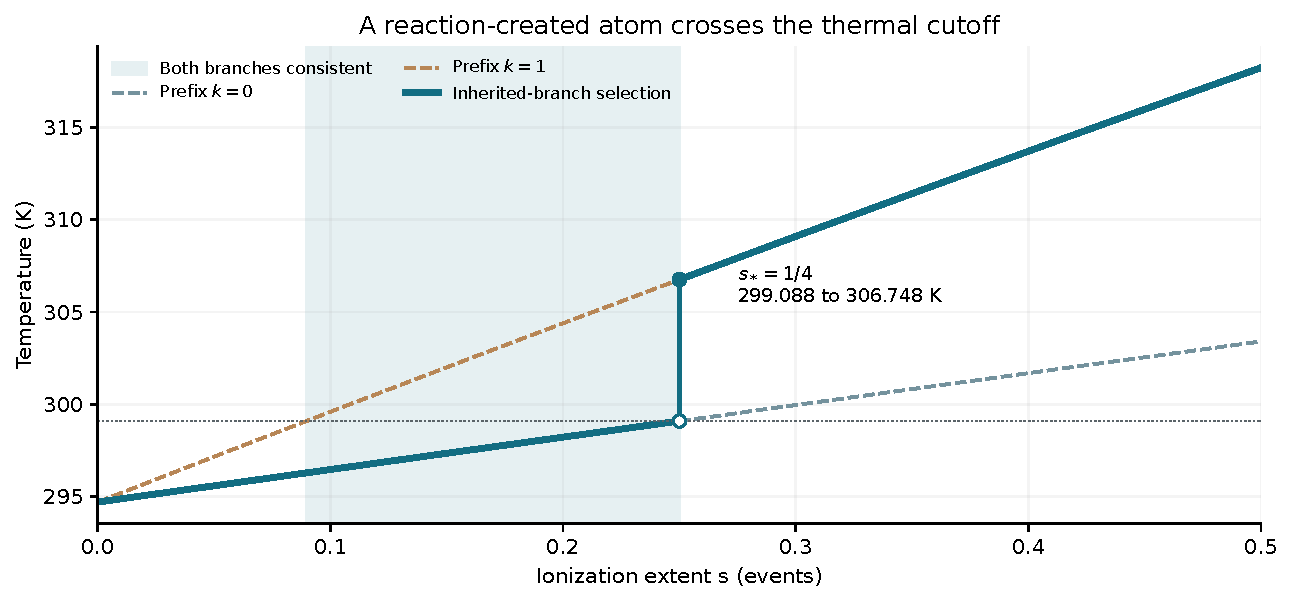
\includegraphics{../figures/reaction_branch.pdf}
\caption{반응 extent에 따라 바뀌는 두 EOS branch. 굵은 선은 지정한 inherited-branch continuation이며, 음영 구간에서는 두 root가 모두 일관적이다.}
\end{figure}

\hypertarget{geometry-uxc774uxb3d9uxacfc-uxc2e4uxc81c-kernel-uxc5f0uxacb0}{%
\section{Geometry 이동과 실제 kernel 연결}\label{geometry-uxc774uxb3d9uxacfc-uxc2e4uxc81c-kernel-uxc5f0uxacb0}}

Massive electron energy는 일반적으로 photon의 \(a^{-1}\) 법칙을 따르지 않는다. 지정된 Bianchi I에서 직교 frame의 운동량을 각 방향의 scale-factor ratio로 옮긴 뒤, mass shell에서 kinetic energy를 계산한다. 모든 방향이 같은 비율로 두 배 팽창한 사례에서는 약 \(30.00977\to7.50261\) eV가 되어 HI/HeI impact threshold 아래로 내려간다. 한 방향이 수축하는 anisotropic 사례에서는 volume이 늘어도 선택한 각분포의 energy가 \(36.67837\) eV로 증가할 수 있다.

\begin{figure}
\centering
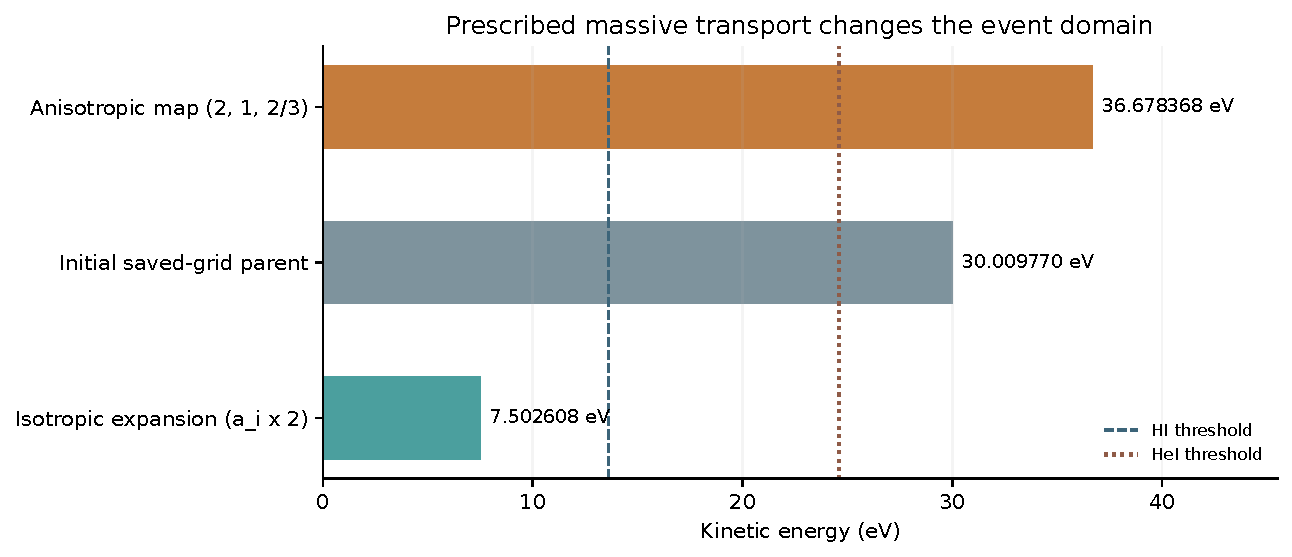
\includegraphics{../figures/geometry_energy.pdf}
\caption{기록된 geometry 사례의 이동 후 에너지와 원 HI/HeI threshold. 방향별 수축을 포함한 경우의 blue shift와 isotropic expansion의 redshift를 구분한다.}
\end{figure}

실제 kernel 재결속은 anisotropic 사례의 moved energy에서 수행했다. HI 17,564개, HeI 13,888개의 새 sharing quadrature가 각각 계산되었고, 각 species에서 actual-subcut·ghost·중간·끝점을 대표하는 4개 contribution을 새 energy row와 함께 구성했다. 이 8개 사건의 수·전하·에너지 장부는 유한 rational arithmetic에서 정확히 보존된다. 전체 sharing을 재평가한 사실과 8개 열을 직접 검사한 사실을 구별한다.

HeI rate \(\kappa(W)=v_{\rm NR}(W)\sigma_{HeI}(W)\)의 한 실제 cell에 대해 분석적인 derivative bound를 세웠다. 현재 cell에서 계산한 \(C^2\) weak bound는 \(2.4279822340661305\times10^{-20}\) m\(^3\)/s, 관측한 FP64 source interpolation error는 \(2.5759954265704087\times10^{-22}\) m\(^3\)/s다. Bound는 frozen finite source parameter를 가진 ideal real scalar 함수의 정리이며, FP64 오차나 전체 branching operator 미분을 대신하지 않는다.

\hypertarget{uxac00uxc815uxc99duxac70uxbb38uxd5ccuxc758-uxc5f0uxacb0}{%
\section{가정·증거·문헌의 연결}\label{uxac00uxc815uxc99duxac70uxbb38uxd5ccuxc758-uxc5f0uxacb0}}

\hypertarget{uxc7acuxc0acuxc6a9uxd55c-uxadfcuxac70}{%
\subsection{재사용한 근거}\label{uxc7acuxc0acuxc6a9uxd55c-uxadfcuxac70}}

직전 branch HEAD는 \nolinkurl{c450b00108dc05885a25d0d9c042cdcfe41bd659}이며, 직전 science commit은 \nolinkurl{a5c29ad4070acb931d92d2bec42a927a57f479ca}다. Copied predecessor source/evidence의 상대경로, bytes, SHA256는 \texttt{inputs/PRIOR\_REUSE.json}에 있다. Accepted event-capacity 보존 증명, 원 kernel, saved energy grid, cutoff의 공통 inventory 정의를 재사용했다. 변경되지 않은 이전 suite를 실행하지 않았다.

\hypertarget{uxc0c8uxb85c-uxc2e4uxd589uxd55c-uxd655uxc778}{%
\subsection{새로 실행한 확인}\label{uxc0c8uxb85c-uxc2e4uxd589uxd55c-uxd655uxc778}}

\begin{longtable}[]{@{}
  >{\raggedright\arraybackslash}p{(\columnwidth - 4\tabcolsep) * \real{0.3333}}
  >{\raggedright\arraybackslash}p{(\columnwidth - 4\tabcolsep) * \real{0.3333}}
  >{\raggedright\arraybackslash}p{(\columnwidth - 4\tabcolsep) * \real{0.3333}}@{}}
\toprule\noalign{}
\begin{minipage}[b]{\linewidth}\raggedright
방법
\end{minipage} & \begin{minipage}[b]{\linewidth}\raggedright
실제 새 확인
\end{minipage} & \begin{minipage}[b]{\linewidth}\raggedright
지지하는 범위
\end{minipage} \\
\midrule\noalign{}
\endhead
\bottomrule\noalign{}
\endlastfoot
Exact-rational reference & coupled endpoint, reaction path, finite ledger & 선언한 finite-input algebra와 domain \\
원 source 함수 & 새 moved HI/HeI sharing, rate, daughter projection & 선택한 energy 및 원 source support \\
Wolfram scalar & 24개 residual 0, 부등식 4개 true & 기재한 scalar 정의와 전제 \\
실제 xAct/xTensor & tensor residual 8개 0 & normalization·spatial constraints 아래 공변 algebra \\
독립 심사 & 후보 proof/code/input/output와 exact identity & 해당 seven scoped claims \\
\end{longtable}

Wolfram 15.0.1 및 xTensor 1.3.0/xPerm 1.2.4의 원 출력이 있다. 공식 xAct 소스의 SHA256를 비교한 후 패키지를 실제로 불러 계산했다. 본문의 수식을 실행하지 않은 notebook으로만 제공한 것이 아니다. Full generator, nonlinear physical ODE integration, NCP job은 이번 단위에서 각각 0건이다.

\hypertarget{uxc6d0uxc804-uxb300uxc870}{%
\subsection{원전 대조}\label{uxc6d0uxc804-uxb300uxc870}}

SciSpace와 Exa를 모두 실제 사용했다. 새 원전 네 편의 관련 절을 읽고, 다음을 비교했다: 상세평형 reaction trajectory scheme의 조건부 유일성; Patankar 계열에서 positivity와 vanishing-component accuracy의 구분; Bianchi I의 covariant momentum과 proper-volume measure; positive conservative characteristic remapping. 원전 정리를 이 후보의 cutoff branch·massive stress 보존에 자동 적용하지 않았다. 완전한 비교와 원 URL은 뒤의 문헌 장에 있다.

\hypertarget{uxc804uxccb4-uxc720uxb3c4uxc640-uxad6cuxd604-uxacc4uxc57d}{%
\section{전체 유도와 구현 계약}\label{uxc804uxccb4-uxc720uxb3c4uxc640-uxad6cuxd604-uxacc4uxc57d}}

이후 네 절에는 새로운 유도, 비자명한 전이의 증명, 실제 입력·계산·오차 해석과 코드 interface를 모두 수록한다. 각 주장에는 식 번호와 결과 파일이 연결된다.

\hypertarget{uxc2e4uxc81c-hi-uxc0acuxac74uxacfc-stoppinguxc744-uxacb0uxd569uxd55c-uxace0uxc815-atomic-branchuxc758-endpoint}{%
\section{실제 HI 사건과 stopping을 결합한 고정 atomic branch의 endpoint}\label{uxc2e4uxc81c-hi-uxc0acuxac74uxacfc-stoppinguxc744-uxacb0uxd569uxd55c-uxace0uxc815-atomic-branchuxc758-endpoint}}

연구 단위: \nolinkurl{CR-THEORY-BRANCH-GEOMETRY-20261013}\\
노드: \nolinkurl{CR_THEORY_COUPLED_BRANCH_SOLVER}\\
현재 기준 Git: \nolinkurl{c450b00108dc05885a25d0d9c042cdcfe41bd659}\\
재사용 근거: KC1--KC7의 실제 saved-grid/kernel 결속, paired event columns, 공통 capacity map, cutoff branch 및 EOS 인터페이스.

\hypertarget{uxc774uxbc88-uxad6cuxc131uxc758-uxbb38uxc81cuxc640-uxc785uxb825}{%
\subsection{이번 구성의 문제와 입력}\label{uxc774uxbc88-uxad6cuxc131uxc758-uxbb38uxc81cuxc640-uxc785uxb825}}

이번에는 실제 source coefficient가 있는 두 사건을 골라, 조성과 thermal electron density가 바뀐 뒤 같은 반응률에 되돌아가는 \textbf{하나의 finite-step endpoint}를 계산한다. 두 사건은 HI full BED sharing의 한 실제 quadrature subchannel과, 별도 active donor의 한 실제 stopping edge다. 초기 재고는 아래에 명시한 \textbf{CONSTRUCTION}이며 historical spectrum을 대신하지 않는다. 선택한 subfamily의 endpoint 존재·유일성·장부·계산오차가 이번 결과다.

원자료는 \nolinkurl{inputs/prior/kernel_event_adapter.py}와 그 아래 source-bound files에서 읽었다. 저장된 9600-node \texttt{energy\_eV} raw digest는 \nolinkurl{6a76d3539115003b046a5861baca89b0a4ff966564627e04d9f6e8bc86be8292}이다. 전체 generator나 이전 physics suite를 재실행하지 않고, 아래 실제 사건과 필요한 stopping coefficient를 결속했다. 입력과 각 source file의 identity는 \nolinkurl{examples/COUPLED_BRANCH_INPUT.json}에 있다.

\begin{longtable}[]{@{}
  >{\raggedright\arraybackslash}p{(\columnwidth - 2\tabcolsep) * \real{0.4286}}
  >{\raggedleft\arraybackslash}p{(\columnwidth - 2\tabcolsep) * \real{0.5714}}@{}}
\toprule\noalign{}
\begin{minipage}[b]{\linewidth}\raggedright
항목
\end{minipage} & \begin{minipage}[b]{\linewidth}\raggedleft
실제 채택값
\end{minipage} \\
\midrule\noalign{}
\endhead
\bottomrule\noalign{}
\endlastfoot
HI parent node & \(j=4762\), \(W_I=30.00976971818039\) eV \\
HI sharing index & \(\ell=38\), 원래 15,620개 quadrature points 중 한 점 \\
실제 sharing probability & \(p_{I}=0.00019359060355166532\) \\
실제 subchannel coefficient & \(\kappa_I=v_I\sigma_H(W_I)p_I=3.336923667758757\times10^{-18}\ {\rm m^3s^{-1}}\) \\
Slow daughter & \(w=0.10194917280817987\) eV \\
Fast daughter & \(W_I-B_H-w=16.30212054537221\) eV \\
HI binding & \(B_H=13.6057\) eV \\
Stopping parent node & \(j=290\), \(W_S=1.00028125\) eV \\
Stopping daughter node & \(j=289\), \(W_D=0.9971875\) eV \\
Stopping heat & \(\delta=W_S-W_D=0.0030937500000000062\) eV \\
\end{longtable}

이 표의 decimal은 사람이 읽는 표시이고, 구현의 source finite inputs와 event columns는 원래 binary rationals로 보존했다. SI energy conversion은 \(\epsilon_{\rm eV}=1.602176634\times10^{-19}\ {\rm J/eV}\), \(k_B=1.380649\times10^{-23}\ {\rm J/K}\), \(c_v=3k_B/2\)다. 원래 비상대론적 source velocity·cold-target stopping prescription을 유지한다.

\hypertarget{uxb450-uxc0acuxac74uxc758-uxc2e4uxc81c-raw-output}{%
\subsection{두 사건의 실제 raw output}\label{uxb450-uxc0acuxac74uxc758-uxc2e4uxc81c-raw-output}}

Source lower absorber는 \(W_b=0.1\) eV이고 첫 active grid node는 \(W_0=0.10309375000000001\) eV다. 선택한 slow daughter는 이 둘 사이에 있다. 따라서 기존 projector는

\[
 \alpha={w-W_b\over W_0-W_b}=0.6300356551692494\ldots,\qquad
 g=1-\alpha=0.3699643448307506\ldots
 \tag{CB.1}
\]

를 사용한다. \(\alpha\) count는 raw node \(A_0\)에, \(g\) count와 \(\epsilon_{\rm eV}W_bg\) energy는 base thermal bath에 들어간다. 이 ghost 분해는 KC의 source projector 자체이며, 그 두 기여의 합은 정확히 한 electron과 \(\epsilon_{\rm eV}w\)다.

Fast daughter는 실제 nodes 3894와 3895, 즉 16.301160463877856 eV와 16.312625762674944 eV 사이에 투영된다. 그 upper barycentric weight를 \(\beta\)라 하자. HI 사건과 stopping 사건의 increments는 다음과 같다.

\begin{longtable}[]{@{}
  >{\raggedright\arraybackslash}p{(\columnwidth - 4\tabcolsep) * \real{0.2727}}
  >{\raggedleft\arraybackslash}p{(\columnwidth - 4\tabcolsep) * \real{0.3636}}
  >{\raggedleft\arraybackslash}p{(\columnwidth - 4\tabcolsep) * \real{0.3636}}@{}}
\toprule\noalign{}
\begin{minipage}[b]{\linewidth}\raggedright
상태
\end{minipage} & \begin{minipage}[b]{\linewidth}\raggedleft
HI 사건 \(S_I\)
\end{minipage} & \begin{minipage}[b]{\linewidth}\raggedleft
Stopping 사건 \(S_S\)
\end{minipage} \\
\midrule\noalign{}
\endhead
\bottomrule\noalign{}
\endlastfoot
\(A_{4762}\) & \(-1\) & 0 \\
\(A_{3894},A_{3895}\) & \(1-\beta,\ \beta\) & 0 \\
\(A_0\) & \(\alpha\) & 0 \\
\(X_{HI},X_{HII}\) & \(-1,+1\) & 0 \\
base thermal electrons \(N_{e,B}\) & \(g\) & 0 \\
base thermal energy \(U_B\) & \(\epsilon_{\rm eV}W_bg\) & \(\epsilon_{\rm eV}\delta\) \\
\(A_{290},A_{289}\) & 0 & \(-1,+1\) \\
\end{longtable}

같은 사건의 모든 coordinate에 하나의 extent를 곱한다. 두 columns는 초기 raw reference에 고정되어 있고, trial temperature나 density에 따라 daughter weights·source energies·초기 donor mask를 변경하지 않는다. Source의 excitation reservoir는 이 subfamily에서 그대로다. HI binding은 \(\epsilon_{\rm eV}B_HX_{HII}\)라는 chemical energy로 한 번 계산한다.

\hypertarget{uxc591uxc758-neutral-uxcd08uxae30-uxc7acuxace0}{%
\subsection{양의 neutral 초기 재고}\label{uxc591uxc758-neutral-uxcd08uxae30-uxc7acuxace0}}

Physical volume과 step을

\[
 V_*=1\ {\rm m^3},\qquad h=10^{14}\ {\rm s}
 \tag{CB.2}
\]

로 고정한다. 두 parent counts는 각각 1이고, 나머지 raw nodes의 초기 count는 0이다. Gas 재고는

\[
 \begin{aligned}
 X_0:=X_{HI}^n&=138.6,\\
 X_{HeI}^n&=11.427127659574467,\qquad X_{HeII}^n=0,\\
 N_{e,B}^n=:n_0&=1.5154255319148937,\\
 X_{HII}^n&=n_0+2.
 \end{aligned}\tag{CB.3}
\]

이다. \(V_*=1\ {\rm m^3}\)이므로 electron count와 수밀도의 수치가 같다. 처음 thermal bath의 전체 particle count는

\[
 N_0=X_0+X_{HII}^n+X_{HeI}^n+N_{e,B}^n
      =155.05797872340426\ldots .
 \tag{CB.4}
\]

초기 \(T_0=100\) K와 \(U_B^n=c_vN_0T_0>0\)를 둔다. 초기 전하는 \(X_{HII}^n-N_{e,B}^n-A_{4762}^n-A_{290}^n=0\)이다. HI 및 thermal electron baseline densities는 원래 source bath의 수치에 맞췄고, 두 active electrons를 포함한 neutrality는 이번 construction에서 별도로 맞췄다. 따라서 전체 nuclei inventory는 historical source 초기조건이라는 주장이 아니다.

큰 \(h\)는 두 피드백과 capacity denominator가 실제로 작동하는 finite-map endpoint를 구성하기 위해 선택했다. 이후의 매우 작은 residual certificate는 이 map의 nonlinear solve 오차에 관한 것이며, \(h\)의 시간 이산화 오차나 전체 물리모형의 정확도에 관한 수치가 아니다.

\hypertarget{extentuxc640-thermal-branchuxc758-uxc815uxd655uxd55c-uxcd95uxc57d}{%
\subsection{Extent와 thermal branch의 정확한 축약}\label{extentuxc640-thermal-branchuxc758-uxc815uxd655uxd55c-uxcd95uxc57d}}

HI extent를 \(x\), stopping extent를 \(s\)라 쓰면 raw endpoint는

\[
 y(x,s)=y^n+xS_I+sS_S.
 \tag{CB.5}
\]

Cutoff closure를 \(E_c=\chi k_BT\), \(\chi=20\)으로 둔다. 고정할 actual grid branch는

\[
 W_{22}=0.17115625\ {\rm eV}
 <{E_c\over\epsilon_{\rm eV}}
 <W_{23}=0.17425000000000002\ {\rm eV}.
 \tag{CB.6}
\]

이 branch에서 raw \(A_0\)는 thermal-owned retained trace이고 다른 occupied raw nodes는 active다. 처음 active donor 둘은 모두 초기 cutoff 위에 있다. 처음 비어 있던 thermal trace를 이후 trial의 새 active donor로 세지 않는다.

\(A_0\)를 base에 중복 합산하지 않고 ownership에 따라 더하면

\[
 \begin{aligned}
 N_{e,th}(x,s)&=n_0+gx+\alpha x=n_0+x,\\
 N_{th}(x,s)&=N_0+x,\\
 U_{th}(x,s)&=c_vN_0T_0+
             \epsilon_{\rm eV}\{(W_bg+W_0\alpha)x+\delta s\}\\
 &=c_vN_0T_0+\epsilon_{\rm eV}(wx+\delta s),\\
 T(x,s)&={c_vN_0T_0+\epsilon_{\rm eV}(wx+\delta s)
                    \over c_v(N_0+x)}.
 \end{aligned}\tag{CB.7}
\]

따라서 반응으로 실제 raw atoms가 생기고 사라지는 동안, 조성·electron bath·thermal count·energy·cutoff가 두 extent에 의해 함께 결정된다. \(N_{e,th}\)는 EOS의 \(N_{th}\)와 구별한다. Density feedback에는 전자를 포함한 전체 active count를 더하지 않는다.

\hypertarget{uxc2e4uxc81c-rateuxc640-uxb450-uxcc28uxc6d0-endpoint-map}{%
\subsection{실제 rate와 두 차원 endpoint map}\label{uxc2e4uxc81c-rateuxc640-uxb450-uxcc28uxc6d0-endpoint-map}}

초기 parent stocks와 positive co-reactant support를 고정하고 trial composition을 rate에 넣으면

\[
 f_I(x)=\kappa_I{X_0-x\over V_*},\qquad
 f_S(x)=\lambda(n_0+x).
 \tag{CB.8}
\]

Stopping source의 \(\alpha_S\)와 baseline Coulomb log를 exact finite inputs로 읽어

\[
 \begin{aligned}
 \lambda(n)&=A_S n L(n),\qquad A_S={\alpha_S\over\delta},\\
 L(n)&=L_0-\tfrac12\log(n/n_0),\\
 A_S&=2.497254955828195\times10^{-9}\ {\rm m^3s^{-1}},\\
 L_0&=29.4116061589828,\qquad
 \lambda(n_0)=1.1130539763458147\times10^{-7}\ {\rm s^{-1}}
 \end{aligned}\tag{CB.9}
\]

로 사용한다. 이는 KC의 thermal bath density continuation이다. Source의 \(\alpha_S,L_0\)를 binary rational로 해석하고 \(\delta\)를 exact grid energy difference로 계산한 baseline rate와 원래 float evaluation의 상대 차이는 \(1.19\times10^{-16}\)이다. 이 rounding 차이는 입력 기록에 명시했다.

두 사건의 negative donors는 각각 \(\{A_{4762},X_{HI}\}\)와 \(\{A_{290}\}\)이고 서로 다른 active parent를 쓴다. 이전 shared-capacity map을 이 두 columns에 적용하면, 새로운 수치기법을 도입하지 않고 정확히

\[
 \Phi_I(x)={a(X_0-x)\over1+b\,a(X_0-x)},\qquad
 \Phi_S(x)={h\lambda(n_0+x)\over1+h\lambda(n_0+x)},
 \tag{CB.10}
\]

\[
 a={h\kappa_I\over V_*}=0.0003336923667758757\ldots,
 \qquad b=1+{1\over X_0},\qquad
 \Phi(x,s)=(\Phi_I(x),\Phi_S(x))
 \tag{CB.11}
\]

을 얻는다. Desired endpoint는 \((x_*,s_*)=\Phi(x_*,s_*)\)다. HI depletion이 첫 rate에, 그 사건이 만드는 thermal electron이 둘째 rate에 실제로 되먹임된다. 이 source의 fixed-energy coefficients에는 직접 \(T\) 인자가 없으므로 temperature는 EOS와 branch 부등식으로 닫힌다. 일반적인 temperature-dependent atomic rate를 인위적으로 추가하지 않았다.

또한 \(z=y^n\)에서 (CB.8)은 원래 source의 해당 selected subchannel 및 stopping rate다. \(h\to0\)이면 \(\Phi_I=h f_I+O(h^2)\), \(\Phi_S=h f_S+O(h^2)\)이고, KC의 fixed-branch first-order consistency가 유지된다.

\hypertarget{uxc22buxc790uxac00-uxc788uxb294-uxb2ebuxd78c-self-map}{%
\subsection{숫자가 있는 닫힌 self-map}\label{uxc22buxc790uxac00-uxc788uxb294-uxb2ebuxd78c-self-map}}

다음 직사각형을 택한다.

\[
 \mathcal D=[0,1/20]\times[0,1],\qquad
 \|(u,v)\|_* =\max(20|u|,|v|).
 \tag{CB.12}
\]

첫 map은 \(x\)에 대해 감소하므로 양 끝만 보면

\[
 0.04417595
 \le\Phi_I(x)\le
 0.04419119
 <0.05.
 \tag{CB.13}
\]

둘째 map의 정의역은 \(n\in[n_0,n_0+0.05]\)다. \(\log(1+r)\le r\)로부터

\[
 L(n)\ge L_0-{0.05\over2n_0}
       =29.395109142485783\ldots>\tfrac12.
 \tag{CB.14}
\]

따라서 \(\lambda>0\), \(\lambda'>0\), \(0<\Phi_S<1\)이다. (CB.13)--(CB.14)는 모두 exact rational inequalities로 확인했으므로 \(\Phi(\mathcal D)\subset\mathcal D\)다.

Thermal closure도 이 domain 전체에서 같은 branch에 남는다. 직접 미분하면

\[
 T_x={N_0(\epsilon_{\rm eV}w-c_vT_0)
                  -\epsilon_{\rm eV}\delta s\over c_v(N_0+x)^2}>0,
 \qquad
 T_s={\epsilon_{\rm eV}\delta\over c_v(N_0+x)}>0.
 \tag{CB.15}
\]

첫 분자의 최소값도 양수다. 따라서

\[
 100\le T(x,s)\le100.376319<100.4\ {\rm K},
 \tag{CB.16}
\]

\[
 0.17234666
 \le {E_c\over\epsilon_{\rm eV}}
 \le0.17299524\quad {\rm eV}.
 \tag{CB.17}
\]

이다. 실제 grid branch의 아래·위 경계까지 균일한 여유는 각각 적어도 \textbf{0.00119041 eV}, \textbf{0.00125476 eV}다. 그러므로 이 self-map의 모든 trial과 endpoint에서 thermal ownership이 유지된다. Source의 lower absorber보다 cutoff가 높으므로 이 구성에는 0.1 eV 아래 trace의 역분류가 요구되지 않는다.

온도 box \([100,100.4]\) K에서 가장 낮은 occupied active node에 대해서도 \(\mathcal W/(k_BT)>115.25\)이다. Positive Coulomb log와 함께 이번 cold-target continuation의 명시된 domain을 확인한다.

\hypertarget{uxc218uxcd95uxb960uxc758-uxc2e4uxc81c-uxc0c1uxacc4}{%
\subsection{수축률의 실제 상계}\label{uxc218uxcd95uxb960uxc758-uxc2e4uxc81c-uxc0c1uxacc4}}

식 (CB.10)의 미분은

\[
 \Phi_I'(x)=-{a\over[1+b\,a(X_0-x)]^2},\qquad
 \Phi_S'(x)={h\lambda'(n_0+x)\over[1+h\lambda(n_0+x)]^2},
 \tag{CB.18}
\]

이고 \(\lambda'(n)=A_S(L(n)-1/2)\), \(\lambda''(n)=-A_S/(2n)<0\)이다. 따라서 \(\lambda\)는 증가하고 \(\lambda'\)는 감소한다. Domain 전체에서

\[
 \begin{aligned}
 q_I&={a\over[1+b\,a(X_0-1/20)]^2}
        =0.0003046579321861247\ldots,\\
 M_S&={h A_S(L_0-1/2)\over[1+h A_S n_0L_0]^2},\\
 q_S&={M_S\over20}=2.9138861430824442\times10^{-9}.
 \end{aligned}\tag{CB.19}
\]

Jacobian의 두 번째 column은 0이다. 그러므로 (CB.12)의 weighted maximum norm에서

\[
 \|\Phi(z)-\Phi(\widetilde z)\|_*
 \le\max(q_I,q_S)\|z-\widetilde z\|_*
 <\bar q\|z-\widetilde z\|_*,\qquad
 \bar q={31\over100000}=0.00031<1.
 \tag{CB.20}
\]

닫힌 완비 self-map에 수축정리를 적용하면 \(\mathcal D\) 안의 endpoint는 존재하고 유일하다. 이 결론은 서로 독립적인 \(T,n_e,X\) 값을 임의로 허용한 box가 아니라, 같은 사건 장부가 정의하는 physical extent domain에서 얻었다. \(T,n_e,X\)는 (CB.5)--(CB.7)의 같은 endpoint에서 함께 복원된다.

\hypertarget{endpointuxc758-uxc2e4uxc81c-uxacc4uxc0b0uxacfc-exact-residual-certificate}{%
\subsection{Endpoint의 실제 계산과 exact residual certificate}\label{endpointuxc758-uxc2e4uxc81c-uxacc4uxc0b0uxacfc-exact-residual-certificate}}

Ion equation은 두 차원 문제에서 먼저 제거할 수 있다. 식 \(x=\Phi_I(x)\)는

\[
 ba x^2-(1+a+baX_0)x+aX_0=0.
 \tag{CB.21}
\]

\(C=1+a(X_0+2)\)라 하면 양의 작은 root를 안정적인 형태로

\[
 x_*={2aX_0\over C+\sqrt{C^2-4a^2(X_0+1)}},\qquad
 C^2-4a^2(X_0+1)=1+2a(X_0+2)+a^2X_0^2>0
 \tag{CB.22}
\]

로 쓸 수 있다. 구현은 \(x=0\)에서 7회의 exact rational scalar update를 수행한 뒤 30 decimal places의 rational \(\widehat x\)를 선택했다. 그 지점에서 stopping log를 아래의 exact enclosure로 계산하고 rational \(\widehat s\)를 선택했다. 이 두 계산 경로는 fixed-point residual로 다시 검증한다.

\(t=x/(2n_0+x)\in[0,1)\)에 대해

\[
 \log\left({n_0+x\over n_0}\right)
 =2\sum_{j=0}^{K-1}{t^{2j+1}\over2j+1}+R_K,
 \quad
 0\le R_K\le{2t^{2K+1}\over(2K+1)(1-t^2)}.
 \tag{CB.23}
\]

이 positive atanh series의 tail bound는 분모를 \(2K+1\)로 낮추고 geometric series를 합해 얻는다. \(K=8\)에서 모든 항과 bound를 Fraction arithmetic으로 계산했다. 따라서 elementary-function floating accuracy에 기대지 않고 \(\Phi_S(\widehat x)\)의 엄밀한 rational interval을 얻는다.

실제 계산한 endpoint 표시는

\[
 \begin{aligned}
 x_*&\simeq0.04417772517583427,\\
 s_*&\simeq0.9999999126593523,\\
 n_{e,*}&\simeq1.559603257090728\ {\rm m^{-3}},\\
 T_*&\simeq100.35047955672445\ {\rm K},\\
 E_{c,*}/\epsilon_{\rm eV}&\simeq0.17295070507127627\ {\rm eV}.
 \end{aligned}\tag{CB.24}
\]

정확한 저장값은 \nolinkurl{examples/COUPLED_BRANCH_ENDPOINT.json}에 있다. \(\widehat z=(\widehat x,\widehat s)\)의 residual과 endpoint bound는

\[
 \eta\ge\|\Phi(\widehat z)-\widehat z\|_*,\qquad
 \|z_*-\widehat z\|_*\le{\eta\over1-\bar q}.
 \tag{CB.25}
\]

실제 exact rational upper bounds는 다음과 같다.

\begin{longtable}[]{@{}lr@{}}
\toprule\noalign{}
Quantity & 검증된 upper bound \\
\midrule\noalign{}
\endhead
\bottomrule\noalign{}
\endlastfoot
Weighted residual \(\eta\) & \(2.153\times10^{-25}\) \\
Endpoint weighted radius & \(2.154\times10^{-25}\) \\
\(x_*\) error & \(1.077\times10^{-26}\) \\
\(T_*\) error & \(8.107\times10^{-26}\) K \\
\end{longtable}

Temperature estimate에는

\[
 L_T\le {\frac1{20}(\epsilon_{\rm eV}w-c_vT_0)
                 +\epsilon_{\rm eV}\delta\over c_vN_0}
      =0.3764399606128681\ldots\ {\rm K}
 \tag{CB.26}
\]

를 썼다. 이는 (CB.15)의 각 partial derivative 최대값을 weighted norm에 맞춰 합한 것이다. \(|T_*-T(\widehat z)|\le L_T\eta/(1-\bar q)\)이고 cutoff error에는 \(\chi k_B/\epsilon_{\rm eV}\)를 더 곱한다.

표의 decimal은 위로 여유를 둔 가독성 표기와 JSON의 exact Fraction certificate를 함께 참조한다. 중요한 정확도는 selected finite-input map의 algebraic solve 정확도다. 원자 자료·source rounding·cold-target closure·시간 적분의 모델 오차는 이 숫자에 포함하지 않는다. Source rounding 비교는 별도 입력 항목으로 남겼다.

\hypertarget{uxc2e4uxc81c-raw-endpointuxc640-uxbcf4uxc874}{%
\subsection{실제 raw endpoint와 보존}\label{uxc2e4uxc81c-raw-endpointuxc640-uxbcf4uxc874}}

저장된 rational approximate endpoint도 \(y^n+\widehat xS_I+\widehat sS_S\)로 조립하므로 invariant는 정확히 유지된다. Endpoint raw inventory는 다음과 같다.

\begin{longtable}[]{@{}
  >{\raggedright\arraybackslash}p{(\columnwidth - 6\tabcolsep) * \real{0.2143}}
  >{\raggedleft\arraybackslash}p{(\columnwidth - 6\tabcolsep) * \real{0.2857}}
  >{\raggedleft\arraybackslash}p{(\columnwidth - 6\tabcolsep) * \real{0.2857}}
  >{\raggedright\arraybackslash}p{(\columnwidth - 6\tabcolsep) * \real{0.2143}}@{}}
\toprule\noalign{}
\begin{minipage}[b]{\linewidth}\raggedright
Raw node
\end{minipage} & \begin{minipage}[b]{\linewidth}\raggedleft
Energy (eV)
\end{minipage} & \begin{minipage}[b]{\linewidth}\raggedleft
Count
\end{minipage} & \begin{minipage}[b]{\linewidth}\raggedright
Endpoint ownership
\end{minipage} \\
\midrule\noalign{}
\endhead
\bottomrule\noalign{}
\endlastfoot
\(A_0\) & 0.10309375000000001 & 0.02783354202504379 & thermal retained trace \\
\(A_{289}\) & 0.9971875 & 0.9999999126593523 & active \\
\(A_{290}\) & 1.00028125 & \(8.7340647674\times10^{-8}\) & active \\
\(A_{3894}\) & 16.301160463877856 & 0.0404783696549195 & active \\
\(A_{3895}\) & 16.312625762674944 & 0.003699355520914768 & active \\
\(A_{4762}\) & 30.00976971818039 & 0.9558222748241657 & active \\
\end{longtable}

Thermal endpoint는 \(N_{th,*}=155.10215644858008\ldots\), \(U_{th,*}=3.2233823978908755\times10^{-19}\) J다. Raw \(A_0\)와 base ghost contribution을 함께 읽어 한 thermal electron per ionization을 회복했다. \(U_B\)와 \(U_{th}\)의 차이를 유지하므로 thermal trace energy를 중복해 더하지 않는다.

보존 rows는 H nuclei, He nuclei, total charge,

\[
 E_{tot}=\epsilon_{\rm eV}\sum_jW_jA_j+U_B
          +\epsilon_{\rm eV}B_HX_{HII}
          +\epsilon_{\rm eV}B_{He}X_{HeII}+E_{exc,H}+E_{exc,He}
 \tag{CB.27}
\]

다. 각각의 두 source event column residual, 실제 endpoint 변화, unchanged capacity map이 만든 state의 변화가 모두 Fraction arithmetic에서 \textbf{정확히 0}이다. 모든 endpoint counts와 energy는 비음수이며 \(U_{th}>0\), \(N_{th}>0\)여서 \(T>0\)이다.

\hypertarget{uxc0c8-uxc2e4uxd589uxacfc-uxb3c5uxb9bd-uxd655uxc778uxc758-uxbc94uxc704}{%
\subsection{새 실행과 독립 확인의 범위}\label{uxc0c8-uxc2e4uxd589uxacfc-uxb3c5uxb9bd-uxd655uxc778uxc758-uxbc94uxc704}}

\nolinkurl{checks/check_coupled_branch.py}는 이번 endpoint에 필요한 새 검사만 수행했다. 실제 실행은 \nolinkurl{results/COUPLED_BRANCH_CHECKS.json}에 UTC, runtime, 당시 input/source hashes와 함께 저장되어 있다.

검사는 먼저 현재 copied source bytes가 결속된 identity와 같은지 확인하고, scalar reduction을 \textbf{변경 없는 이전 \texttt{capacity\_step}}에 두 source columns와 trial rates를 직접 넣은 결과와 비교했다. Ion extent는 exact equality이며 stopping extent는 (CB.23)의 rigorous enclosure 안에 있다. 이어 (CB.21)의 polynomial이 certified \(x\)-interval 양 끝에서 각각 비음수와 비양수이고 그 안에서 strictly decreasing임을 확인했다. 이는 수축 estimate와 별도의 exact algebraic enclosure다.

Domain corners와 endpoint의 raw inventory를 직접 분류하여 (CB.7)의 count·energy 응답을 확인했다. 증명에서 쓰인 self-map, branch margin, positive log와 \(\bar q<1\) 부등식은 모두 rational comparisons로 계산했다. 이전 full generator·ODE·NCP 또는 기존 suite는 호출하지 않았다.

Root가 수행한 새 Wolfram scalar 검산에서도 ion-map derivative, fixed-point quadratic, stable small root·discriminant, \(T_x,T_s\), stopping의 1·2차 미분과 map derivative, atanh log-ratio 미분이 exact zero residual로 확인되었다. 그 실행 근거는 root의 \nolinkurl{checks/wolfram_branch_geometry_scalar.wl} 및 \nolinkurl{results/WOLFRAM_SCALAR_RAW.json}에 결속된다. \nolinkurl{examples/COUPLED_BRANCH_WOLFRAM_INPUT.json}은 숫자 결속용 보조 자료이며, 실제 Wolfram 실행 입력은 \nolinkurl{checks/wolfram_branch_geometry_scalar.wl}의 일반기호식과 전제다. 실제 실행 범위는 일반기호식 24개와 부등식 4개이며, 이 JSON의 숫자를 Wolfram에 주입하지 않았다.

실행 이후 채택 근거 라벨의 \texttt{KC1-KC8} 오기를 \texttt{KC1-KC7}로 교정했다. 과학 식·수치 입력·결과는 바뀌지 않았고, 당시 실행 identity는 CHECKS 파일에 그대로 남겼다. 현재 metadata가 달라진 의미와 변경 전후 hashes는 \texttt{results/COUPLED\_BRANCH\_METADATA\_PATCH.json}에 별도로 기록한다. 이 label 교정을 위해 science를 다시 실행하지 않았다.

\hypertarget{uxb2ebuxd78c-uxacb0uxacfcuxc640-uxb2e4uxc74c-uxc5f0uxacb0}{%
\subsection{닫힌 결과와 다음 연결}\label{uxb2ebuxd78c-uxacb0uxacfcuxc640-uxb2e4uxc74c-uxc5f0uxacb0}}

이번 분과에서 실제 source-bound selected subfamily에 대해 다음 연결을 완성했다: 초기 positive neutral stock → 고정 source columns → trial HI density와 thermal electron density → common capacity extents → reaction-changed raw atoms → 같은 atomic branch의 thermal EOS → unique endpoint와 residual certificate.

Root의 reaction-driven crossing construction은 같은 HI source event에 다른 \(\chi\)와 초기 재고를 둔 별도 문제다. 여기의 \(\chi=20\) self-map에서는 명시한 양의 margins 때문에 crossing이 일어나지 않는다. 이 조건을 제거해 branch를 이동시키는 문제는 root의 conservative crossing 결과와 연결한다. Geometry 뒤 actual parent energy가 변하는 경우에는 다른 분과의 off-grid source rebinding이 새 immutable columns를 제공한다. 그 다음에 동일한 domain·ownership·rate-bound 계약을 다시 평가하면 된다.

Full HI sharing family, 나머지 물리 channels, 온도 의존적인 finite-temperature rate closure 및 실제 time-accuracy budget은 이 두 사건의 algebraic endpoint certificate와 구별한 후속 범위다. 현재 결과는 그 후속 계산에 재사용할 수 있는 구체적인 positive conservative coupled endpoint와 수치가 있는 self-map/error contract다.

\clearpage

\hypertarget{uxbc18uxc751uxc73cuxb85c-uxc6d0uxc790-uxac00uxc911uxce58uxac00-uxbc14uxb00cuxb294-uxc720uxd55c-cutoff-branch-uxad6cuxc131}{%
\section{반응으로 원자 가중치가 바뀌는 유한 cutoff branch 구성}\label{uxbc18uxc751uxc73cuxb85c-uxc6d0uxc790-uxac00uxc911uxce58uxac00-uxbc14uxb00cuxb294-uxc720uxd55c-cutoff-branch-uxad6cuxc131}}

\hypertarget{uxacb0uxacfcuxc640-uxbc94uxc704}{%
\subsection{결과와 범위}\label{uxacb0uxacfcuxc640-uxbc94uxc704}}

고정된 유한 에너지 support에서 반응이 원자 가중치, 기저 전자 수, 기저 열에너지와 이온 조성을 동시에 바꾸어도, 각 raw state의 cutoff branch를 \textbf{이전 branch에서 시작하는 유한 scan}으로 선택할 수 있다. 아래 정리는 \(\chi\ge3/2\), 양의 기저 열용량과 비음수 raw 원자 가중치 아래 성립한다. 한 raw state에서 최대 원자 수만큼 이동하며, 선택한 열/비열 장부의 수와 에너지 합은 변하지 않는다. 반응 경로 전체의 유일한 EOS 해를 가정하지 않는다.

실제 PHYS02C HI kernel의 한 sharing contribution을 사용하여, 반응이 새로 만드는 첫 energy-grid 원자의 가중치가 증가하다가 cutoff에 편입되는 예제를 완성했다. 같은 반응 extent에서 두 consistent branch도 실제로 존재한다. 따라서 inherited branch는 반복 알고리즘의 편의값이 아니라 이 유한 표현의 \textbf{명시적인 선택 입력}이다.

이 절의 예제는 구성한 초기 재고와 하나의 source-pinned quadrature contribution에 대한 결과다. 선택한 contribution의 원래 확률은 rate coefficient 안에 유지하며, 선택 후 확률을 1로 재정규화하지 않는다. 시간 \(h\)는 accepted capacity map의 step parameter이며, nonlinear kinetic ODE의 정확한 경과 시간이나 cosmological history 정확도로 해석하지 않는다.

\hypertarget{uxbcc0uxd654uxd558uxb294-uxacf5uxd1b5-raw-inventory}{%
\subsection{변화하는 공통 raw inventory}\label{uxbcc0uxd654uxd558uxb294-uxacf5uxd1b5-raw-inventory}}

서로 다른 고정 에너지 \(0<w_1<\cdots<w_M\), raw 원자 가중치 \(a_j(s)\ge0\), 기저 입자 수 \(N_B(s)>0\), 기저 열에너지 \(U_B(s)>0\)를 둔다. 에너지는 J, 수는 같은 물리 cell의 count이며 \(s\)는 반응 extent이다. \(k_B\)는 SI 상수,

\[c_v=\frac32 k_B,\qquad \alpha=\chi k_B,\qquad E_c(T)=\alpha T.\tag{RB.1}\]

기저 수에는 모든 열적 nuclei와 unresolved thermal electrons가 들어간다. retained raw 원자는 소유가 thermal인지 active인지와 무관하게 \(a_j\)에 한 번 저장하고, \(N_B,U_B\)에서 그 수와 에너지를 다시 빼고 더하지 않는다. 원 source의 0.1 eV absorber/ghost에 포함된 전자는 이 예제에서 기저에 남는다. 모든 채택 cutoff가 그 absorber보다 높다는 조건을 아래에서 검증한다.

앞에서부터 \(k\)개를 thermal로 분류하면

\[N_k=N_B+\sum_{j\le k}a_j,\quad U_k=U_B+\sum_{j\le k}w_ja_j,\quad T_k=\frac{U_k}{c_vN_k}.\tag{RB.2}\]

\(w_0=0,w_{M+1}=\infty\)로 두었을 때 branch 일관성은

\[w_k\le\alpha T_k<w_{k+1}.\tag{RB.3}\]

등호는 thermal 소유다. Support에 가중치 0인 항을 유지해도 수/에너지는 변하지 않는다. 같은 에너지의 항은 먼저 하나로 합친다. 반응이 새로운 에너지를 만들면 현재 단계의 모든 사건 열이 만드는 support의 합집합을 먼저 고정한다. 에너지 자체의 geometry 이동은 별도 geometry map에서 처리한 후 이 단계의 support로 고정한다.

고정 \(k\)에서 \(C^1\)인 raw path의 미분은

\[\frac{dT_k}{ds}=\frac{U'_B+\sum_{j\le k}w_ja'_j-c_vT_k(N'_B+\sum_{j\le k}a'_j)}{c_vN_k}.\tag{RB.4}\]

따라서 기존의 \(U_B\)만 바뀌는 공식에 비해, 반응으로 변하는 \textbf{원자 가중치와 기저 수}가 모두 들어간다. 이 식은 cutoff를 미리 smooth하게 만든 유도가 아니며, 고정 prefix 내부의 정확한 미분이다.

\hypertarget{uxd55c-raw-stateuxc758-uxc720uxd55c-scan-uxc815uxb9ac}{%
\subsection{한 raw state의 유한 scan 정리}\label{uxd55c-raw-stateuxc758-uxc720uxd55c-scan-uxc815uxb9ac}}

입력 inherited index를 \(k\)라 한다. 현재 \(T_k\)가 lower condition을 위반하면 가장 높은 thermal 원자를 제거한다. 그렇지 않고 upper condition을 위반하면 가장 낮은 active 원자를 추가한다. 일관성을 만족하면 종료한다.

\hypertarget{uxcd94uxac00-uxb2e8uxacc4}{%
\subsubsection{추가 단계}\label{uxcd94uxac00-uxb2e8uxacc4}}

다음 원자 \((w,a)\)가 \(w\le\alpha T_k\)를 만족하면

\[\alpha T_{k+1}=\frac{N_k\alpha T_k+(\alpha/c_v)aw}{N_k+a}\ge w,\qquad\frac\alpha{c_v}=\frac{2\chi}3\ge1.\tag{RB.5}\]

이미 들어 있던 에너지는 모두 \(w\) 이하이므로 lower consistency가 유지된다. 추가 후 온도가 감소하는 경우에도 이 부등식은 성립한다. 다음 upper violation에 대해서만 같은 단계를 반복하면 유한 \(M\)회 이내에 종료한다. 모든 원자를 넣었으면 upper bound는 \(\infty\)다.

\hypertarget{uxc81cuxac70-uxb2e8uxacc4}{%
\subsubsection{제거 단계}\label{uxc81cuxac70-uxb2e8uxacc4}}

가장 높은 thermal 원자가 \(w>\alpha T_k\)를 만족하면 \(w>c_vT_k\)이므로

\[T_{k-1}-T_k=\frac{a(c_vT_k-w)}{c_v(N_k-a)}\le0.\tag{RB.6}\]

분모는 최소 \(N_B>0\)이다. 제거한 원자는 새 cutoff 위에 있고, 앞서 제거한 더 높은 원자도 모두 위에 남는다. Lower violation이 없어질 때까지 제거하면 유한 \(M\)회 이내에 종료한다. \(k=0\)에서는 \(T_0>0\)이므로 lower condition을 만족한다.

따라서 한 raw state의 scan은 방향을 되돌릴 필요가 없고, 양의 EOS와 비음수 원자 수를 보존한다. 분류가 바뀔 때마다 동일한 실제 원자 에너지를 옮기므로

\[N_{\rm th}+N_{\rm act}=N_B+\sum_j a_j,\qquad U_{\rm th}+U_{\rm act}=U_B+\sum_jw_ja_j\tag{RB.7}\]

는 정확히 불변이다. 다른 chemical/excitation reservoir는 분류에 의해 변하지 않는다. 반응에 따른 물리 변화는 raw state를 만드는 공통 사건 열에서 이미 계산된다.

이는 한 endpoint의 유한 종료 정리다. 임의의 진동하는 \(C^1\) parameter path 전체가 유한 횟수만 교차한다는 주장은 아니다. 전체 continuation을 유한 event sequence로 인증하려면 해당 경로의 교차 수, transversality와 event separation을 별도로 확인해야 한다.

\hypertarget{uxad50uxcc28uxba74uxacfc-uxc628uxb3c4-jump}{%
\subsection{교차면과 온도 jump}\label{uxad50uxcc28uxba74uxacfc-uxc628uxb3c4-jump}}

Branch \(k\)의 상단에서

\[b_k(s)=\alpha U_k(s)-c_vw_{k+1}N_k(s)\tag{RB.8}\]

를 정의한다. \(b_k<0\)가 upper consistency다. \(b_k(s_*)=0\), \(b'_k(s_*)>0\), \(a_{k+1}(s_*)>0\)이면 increasing parameter 방향에서 inherited branch가 이 상단을 통과한다. 교차 시점의 추가는

\[\Delta T=\frac{a_{k+1}(w_{k+1}-c_vT_k)}{c_v(N_k+a_{k+1})}
=\frac{a_{k+1}w_{k+1}(1-c_v/\alpha)}{c_v(N_k+a_{k+1})}\ge0.\tag{RB.9}\]

\(\chi>3/2\)와 양의 crossing weight이면 엄밀히 양수다. 첫 추가가 그다음 경계도 넘으면 RB.5로 cascade를 끝까지 수행한다. \(\chi=3/2\)에서는 이 경계 jump가 0이다. 반대 방향 lower crossing의 제거 jump는 RB.6으로 정해진다. 양의 atom weight에서 나타나는 이 온도 jump는 \textbf{선택한 유한 sharp-cutoff EOS의 분류 변화}이며, 실제 물리 온도가 순간적으로 불연속이라는 증거가 아니다.

\hypertarget{uxc2e4uxc81c-hi-contributionuxc5d0-uxacb0uxc18duxd55c-uxad6cuxc131}{%
\subsection{실제 HI contribution에 결속한 구성}\label{uxc2e4uxc81c-hi-contributionuxc5d0-uxacb0uxc18duxd55c-uxad6cuxc131}}

재사용한 kernel identity는 \nolinkurl{inputs/prior/inputs/KERNEL_SOURCE_BINDING.json}에 고정되어 있다. Parent는 저장된 9600-grid의 Python index 4762,

\[W_p=30.00976971818039\ {\rm eV},\qquad B_H=13.6057\ {\rm eV}.\tag{RB.10}\]

원 sharing index 38의 느린 daughter는 \(w_s=0.10194917280818\) eV, 빠른 daughter는 약 16.3021205453722 eV다. 원 quadrature 확률을 포함한 coefficient는 약 \(\kappa=3.336923667758757\times10^{-18}\) m\(^3\) s\(^{-1}\)다. 정확히 사용한 finite-binary rational은 결과 JSON에 보존한다.

느린 daughter가 source absorber \(w_c=0.1\) eV와 첫 grid node \(w_1=0.10309375\) eV 사이에 있으므로 원 projector는

\[g=\frac{w_1-w_s}{w_1-w_c},\qquad a=1-g=\frac{w_s-w_c}{w_1-w_c}\tag{RB.11}\]

의 ghost와 첫 node로 분해한다. 두 항의 합은 정확히 1이고 \(g w_c+a w_1=w_s\)다. \(g\)는 기저 thermal count, \(g w_c\)는 그 열에너지에 들어간다. 이 contribution에는 actual-subcut daughter가 없다. 빠른 daughter의 원 barycentric 두 node도 raw state에 유지한다.

별도 구성 초기 재고를 \(V=1\) m\(^3\), \(N_{HI}=7\), \(N_{HII}=2\), \(N_{e,B}=1\), active parent count 1로 둔다. 따라서 nuclei는 9, \(N_B^0=10\)이며 ion charge 2와 자유전자 count 2가 일치한다. 초기 raw 첫 node와 빠른 daughter의 가중치는 0이다. \(\chi=4\), \(s_*=1/4\)로 두고 SI로 변환한 \(w_c,w_1\)을 사용하여

\[U_B^0=\frac{c_v}{\alpha}w_1N_B^0-g\left(w_c-\frac{c_v}{\alpha}w_1\right)s_*\tag{RB.12}\]

로 초기 열에너지를 \textbf{구성한다}. 이 값은 양수이고 초기 cutoff는 \(w_c\)와 \(w_1\) 사이에 있다.

동일한 ionization event 열 \(S\)를 하나의 extent \(s\)로 갱신하면

\[y(s)=y^0+sS,\quad N_B(s)=10+gs,\quad U_B(s)=U_B^0+gw_cs,\quad a_1(s)=as.\tag{RB.13}\]

또한 parent는 \(1-s\), HI는 \(7-s\), HII는 \(2+s\), 빠른 daughter count는 \(s\)다. 기저/첫 node/빠른 daughter를 합친 자유전자 수는 반응 한 번당 1 증가한다. Chemical energy는 \(B_Hs\)만큼 증가한다. 실제 사건 열을 그대로 사용하므로 총 kinetic+chemical energy, H/He nuclei와 charge의 네 invariant residual은 모든 계산점에서 정확히 0이다.

Branch 0의 상단 함수는

\[b_0(s)=g(\alpha w_c-c_vw_1)(s-s_*),\qquad g(\alpha w_c-c_vw_1)>0.\tag{RB.14}\]

따라서 생성된 원자 가중치가 \(a/4>0\)인 상태에서 정확히 \(s=1/4\)에 첫 node가 편입된다. 그 뒤 첫 node까지 포함한 분자는 \(U_B^0+w_ss\), 분모의 count는 \(10+s\)다.

\hypertarget{uxc2e4uxc81c-uxc870uxc131-feedback-uxbc0f-step-parameter}{%
\subsection{실제 조성 feedback 및 step parameter}\label{uxc2e4uxc81c-uxc870uxc131-feedback-uxbc0f-step-parameter}}

초기 parent count 1과 초기 neutral count 7을 capacity denominator에 유지하고, trial neutral은 실제 endpoint \(7-s\)를 쓰면

\[f(s)=\kappa\frac{7-s}{V},\qquad \Psi_h(s)=\frac{hf(s)}{1+(8/7)hf(s)}.\tag{RB.15}\]

아래에서는 \(V=1\) m\(^3\)의 count convention이다. 지정한 \(0\le s<7/8\)에 대해

\[h(s)=\frac{sV}{\kappa(7-s)[1-(8/7)s]}\tag{RB.16}\]

를 선택하면 \(s=\Psi_{h(s)}(s)\)가 정확히 성립한다. 이것은 frozen neutral의 단순 평가가 아니라 이 subfamily의 조성 feedback을 닫은 식이다. \(h>0\)에서 \(\Psi_h\)는 감소하고 \(s\)는 증가하므로 그 교점은 유일하다. \([0,1]\)에 대한 \(\Psi_h\)의 image는 \([0,7/8)\) 안에 있어 존재한다. 이 유일성은 extent에 관한 것이며 cutoff branch의 유일성과 다르다.

\(0\le s\le1/2\)에 결속한 \(h\le h(1/2)\)에서는 \(a_h=h\kappa/V\le7/39\simeq0.17949\)이고

\[|\Psi'_h(s)|=\frac{a_h}{[1+(8/7)a_h(7-s)]^2}\le a_h<1\qquad(0\le s\le1).\tag{RB.17}\]

따라서 해당 domain에서 일반 fixed-point defect의 extent error는 \(|\widehat s-\Psi_h(\widehat s)|/(1-a_h)\)로 제한할 수 있다. 아래 예제는 RB.16의 정확 rational \(h\)를 써 defect 자체가 0이다.

\hypertarget{uxc0c8-uxc2e4uxd589-uxacb0uxacfcuxc640-uxd310uxbcc4}{%
\subsection{새 실행 결과와 판별}\label{uxc0c8-uxc2e4uxd589-uxacb0uxacfcuxc640-uxd310uxbcc4}}

\nolinkurl{python3 checks/check_reaction_branch.py}를 새로 실행했다. 0, 1/5, 1/4, 3/10, 1/2의 다섯 extent에서 같은 initial state와 source event로 raw state를 독립 구성했다. Fraction arithmetic은 \textbf{사용한 유한 source 숫자}에 대한 대수적 정확성을 인증한다. 원 cross section의 물리 정확도나 원 quadrature 오차를 0이라고 만들지 않는다.

\begin{longtable}[]{@{}lr@{}}
\toprule\noalign{}
새 판별량 & 실제 결과 \\
\midrule\noalign{}
\endhead
\bottomrule\noalign{}
\endlastfoot
초기 온도 & 294.6991929990844 K \\
교차 extent & 정확히 1/4 \\
교차의 capacity step parameter & \(1.5538818688854852\times10^{16}\) s \\
교차 직전 branch 0 온도 & 299.0883225233885 K \\
동일 raw state의 선택 branch 1 온도 & 306.7483350125956 K \\
교차 뒤 cutoff & 0.10573410521646769 eV \\
그 순간 편입되는 생성 원자 수 & 0.15750891379231236 \\
네 invariant 및 extent 식 residual & 각 계산점에서 정확히 0 \\
\end{longtable}

동일한 \(s=1/5\)에서 branch 0과 branch 1이 모두 RB.3을 만족한다. Branch 1의 lower consistency 시작점은

\[s_- =\frac{c_vw_1N_B^0-\alpha U_B^0}{\alpha w_s-c_vw_1}
\simeq0.08964254913065285 <\frac15<\frac14.\tag{RB.18}\]

이는 동일 extent의 root multiplicity를 직접 보여준다. 현재 선택은 inherited branch 0을 유지하다가 upper equality에서 branch 1로 넘어가는 continuation이다. 반대 경로를 물리적인 역이온화 계산으로 실행한 것은 아니다. 이 결과를 새 strong no-go로 채택하지 않으며, 실제로 완성한 유한 선택 규칙과 반응 예제로 보존한다.

\hypertarget{uxb2e4uxc74c-uxc758uxbb34}{%
\subsection{다음 의무}\label{uxb2e4uxc74c-uxc758uxbb34}}

여러 실제 family의 rate가 cutoff branch별 \(n_e,T\)에 다시 의존하면 서로 다른 branch에서 extent 자체도 달라질 수 있다. 그 경우 branch별 coupled domain/error certificate와 crossing compatibility를 함께 구해야 한다. 이 루프의 별도 fixed-branch 구성은 그중 한 separated domain을 닫는다. 전체 multi-family crossing continuation의 전역 유일성, step refinement 및 유한 spectral representation을 연속 spectrum과 비교하는 오차는 다음 DAG 의무로 남긴다.

근거: \nolinkurl{reaction_branch_continuation.py}, \nolinkurl{checks/check_reaction_branch.py}, \nolinkurl{results/REACTION_BRANCH_CHECKS.json}, accepted predecessor의 KA/TCF/CP 유도. 문헌과 현재 정리의 적용 범위 대응은 \texttt{LITERATURE\_KO.md}에 모은다.

\clearpage

\hypertarget{uxc9c8uxb7c9-uxc788uxb294-uxc804uxc790uxc758-prescribed-bianchi-uxc5d0uxb108uxc9c0-uxc774uxb3d9}{%
\section{질량 있는 전자의 prescribed Bianchi 에너지 이동}\label{uxc9c8uxb7c9-uxc788uxb294-uxc804uxc790uxc758-prescribed-bianchi-uxc5d0uxb108uxc9c0-uxc774uxb3d9}}

\hypertarget{uxacb0uxacfcuxc640-uxbb3cuxb9ac-convention}{%
\subsection{결과와 물리 convention}\label{uxacb0uxacfcuxc640-uxbb3cuxb9ac-convention}}

Signature는 \((-+++)\), \(n^an_a=-1\), \(n^a\)는 미래 방향의 unit cosmological normal이다. \(c,\hbar,k_B\)를 1로 놓지 않는다. 아래 classical geodesic 운동식에는 \(\hbar\)가 나타나지 않고, 원 collision/stopping kernel의 양자 상수 convention은 그대로 유지한다. Geometry는 지정된 배경 입력이고 Einstein 방정식을 이 절에서 풀지 않는다.

전자 질량을 \(m_e\), 관측 총에너지를 \(E=m_ec^2+W\)라 쓰면, 동기화된 geodesic normal의 homogeneous Bianchi 배경에서

\[\frac{dW}{dt}=-\frac{c^2}{E}K_{ab}q^aq^b
=-\frac{W(W+2m_ec^2)}{W+m_ec^2}\left(H+\sigma_{ab}e^ae^b\right).\tag{BG.1}\]

여기서 \(q^a\)는 normal에 수직인 물리 운동량, \(e^a=q^a/|q|\)이고 \(W>0\)에서 두 번째 식을 쓴다. \(W=0\)에서는 첫 식이 잘 정의되어 drift가 0이다. \(K_{ab}=H\gamma_{ab}+\sigma_{ab}\)는 단위가 s\(^{-1}\)인 팽창률 tensor이다. 양의 \(H\)가 팽창을 뜻하도록 부호를 고정하며, 다른 ADM extrinsic-curvature 부호 관례를 그대로 대입하지 않는다.

\hypertarget{uxacf5uxbcc0-uxc720uxb3c4}{%
\subsection{공변 유도}\label{uxacf5uxbcc0-uxc720uxb3c4}}

공간 projector와 momentum 분해를

\[\gamma_{ab}=g_{ab}+n_an_b,\qquad p^a=\frac Ec n^a+q^a,\qquad n_aq^a=0,\qquad E=-cn_ap^a\tag{BG.2}\]

로 정의한다. 질량껍질 \(p^ap_a=-m_e^2c^2\)에서

\[c^2q^aq_a=E^2-m_e^2c^4=W(W+2m_ec^2).\tag{BG.3}\]

Geodesic \(p^a\nabla_ap^b=0\)와 product rule을 사용하면

\[p^a\nabla_aE=-c p^ap^b\nabla_an_b.\tag{BG.4}\]

동기화된 cosmological proper time \(t\)는 \(\nabla_at=-n_a/c\)이므로 \(p^a\nabla_at=E/c^2\)다. 따라서

\[\frac{dE}{dt}=-\frac{c^3}{E}p^ap^b\nabla_an_b.\tag{BG.5}\]

일반 observer normal에 대한 분해를 잠시 쓰면

\[\nabla_an_b=-n_a a_b+\frac1cK_{ab},\qquad n^aa_a=0,\quad n^aK_{ab}=0\tag{BG.6}\]

이며 \(a_b=n^a\nabla_an_b\)의 단위는 m\(^{-1}\)다. Vorticity가 없는 normal을 전제로 썼다. 같은 contraction은 local observer clock \(dt_{\rm obs}=-n_a dx^a/c\)에 대해

\[\frac{dE}{dt_{\rm obs}}=-c^2 a_bq^b-\frac{c^2}{E}K_{ab}q^aq^b\tag{BG.7}\]

를 준다. Accelerated observer에서는 이 local clock을 전역 cosmological time의 gradient라고 가정하지 않는다. 본 연구의 synchronous homogeneous Bianchi normal에서는 \(a_b=0\)이고 \(K_{ab}=c\nabla_an_b\)여서 BG.5--7이 BG.1의 첫 식으로 줄어든다. \(K=H\gamma+\sigma\)와 BG.3을 대입하면 두 번째 식을 얻는다.

삼차원 frame 회전의 반대칭 계수 \(\Omega_{ab}\)는 \(\Omega_{ab}q^aq^b=0\)이므로 scalar work를 직접 만들지 않는다. 일반 Bianchi 유형의 구조상수와 frame transport는 \(q^a\)의 방향 변화에 관여한다. 따라서 BG.1의 순간 scalar 법칙만으로 모든 Bianchi 유형의 방향 경로까지 얻었다고 주장하지 않는다.

\hypertarget{uxbe44uxc0c1uxb300uxb860-uxadf9uxd55cuxacfc-uxc9c8uxb7c9-uxc5c6uxb294-uxadf9uxd55c}{%
\subsection{비상대론 극한과 질량 없는 극한}\label{uxbe44uxc0c1uxb300uxb860-uxadf9uxd55cuxacfc-uxc9c8uxb7c9-uxc5c6uxb294-uxadf9uxd55c}}

\(R=m_ec^2\)로 쓰면

\[\frac{W(W+2R)}{W+R}=2W-\frac{W^2}{W+R}.\tag{BG.8}\]

\(W/R\ll1\)일 때 \(\dot W=-2W(H+\sigma ee)+O(W^2|H+\sigma ee|/R)\)다. 고정된 방향 rate에 대해 leading nonrelativistic work와 exact work의 차이는 정확히 \(W^2|H+\sigma ee|/(W+R)\)다. Isotropic 경우 비상대론 kinetic energy가 \(a^{-2}\)로 줄어드는 것은 이 식의 극한이다. Massless limit \(R\to0\)에서는 \(\dot E=-E(H+\sigma ee)\)를 회복한다.

원 BASS\_CR ionization rate가 사용하는 \(v_{\rm NR}=\sqrt{2W/m_e}\)는 그대로 둔다. 본 절에서 kinematics를 정확한 massive form으로 썼다는 사실은 기존 atomic cross section이나 그 nonrelativistic speed 모델의 물리 정확도를 바꾸지 않는다. 새 에너지에서 source 함수를 다시 평가하고 그 원 domain을 유지한다.

\hypertarget{bianchi-iuxc5d0uxc11c-uxc2e4uxc81c-uxc720uxd55c-geometry-map}{%
\subsection{Bianchi I에서 실제 유한 geometry map}\label{bianchi-iuxc5d0uxc11c-uxc2e4uxc81c-uxc720uxd55c-geometry-map}}

Diagonal Bianchi I metric

\[ds^2=-c^2dt^2+\sum_{i=1}^3 a_i(t)^2(dx^i)^2,\quad a_i(t)>0\tag{BG.9}\]

의 spatial Killing directions에서 covariant coordinate momentum \(P_i=a_iq_{\hat i}\)가 일정하다. 여기서 \(q_{\hat i}\)는 직교 frame의 물리 momentum이다. 따라서 두 지정 시점 사이에서

\[q_{\hat i}^{\,+}=r_iq_{\hat i}^{\,-},\qquad r_i=\frac{a_i(t_-)}{a_i(t_+)}>0,\qquad
E^+=\sqrt{m_e^2c^4+c^2\sum_i(q_{\hat i}^{\,+})^2}.\tag{BG.10}\]

이는 prescribed Bianchi I의 collision-free geodesic map이다. 일반 Bianchi에서 covariant spatial momenta가 모두 상수라는 가정으로 확장하지 않는다. BG.10을 미분하여 \(H_i=\dot a_i/a_i\)를 쓰면 \(\dot W=-\sum_iH_i c^2q_{\hat i}^2/E\)가 되며 BG.1과 일치한다.

낮은 kinetic energy에서 \(E-R\)의 cancellation을 피하기 위해

\[W^+=\frac{p_c^{+\,2}}{\sqrt{R^2+p_c^{+\,2}}+R},\qquad p_c^+=c|\mathbf q^+|\tag{BG.11}\]

를 쓴다. 실제 구현은 \texttt{hypot}와 이 rationalized 식으로 FP64 geometry energy를 얻고, 그 \textbf{유한 계산값}을 exact rational 장부에 넣는다. Rational 장부의 보존은 FP64 geometry 해석 오차를 0으로 만드는 것이 아니다. 별도 high-precision scalar 비교로 작은 입력 오차를 관찰하고, projection의 representation 오차와 구분한다.

\hypertarget{uxc218-pressure-work-cutoff-uxc774uxb3d9uxc758-uxc7a5uxbd80}{%
\subsection{수, pressure work, cutoff 이동의 장부}\label{uxc218-pressure-work-cutoff-uxc774uxb3d9uxc758-uxc7a5uxbd80}}

고정 comoving cell의 packet counts \(N_j\)와 raw angular energies를 보유하면 geometry map에서 \(N_j^+=N_j^-\)다. Kinetic energy 변화는

\[\Delta U_{\rm geom}=\sum_jN_j(W_j^+-W_j^-).\tag{BG.12}\]

지정된 배경과의 work를 기록하는 signed accumulator \(G^+=G^- -\Delta U_{\rm geom}\)를 두면 \(U_{\rm packets}+G\)는 이 단계의 정확한 장부 invariant다. \(G\)는 배경의 work accumulator이며 국소적인 중력 에너지 tensor나 일반 시공간의 전역 보존 에너지를 정의한 것이 아니다. \(\Delta U_{\rm geom}\)를 thermal collision heat로 동시에 더하지 않는다.

물리 volume \(V\propto a_1a_2a_3\)와

\[P^{ab}=\frac1V\sum_jN_j\frac{c^2q_j^aq_j^b}{E_j},\quad u_A=\frac1V\sum_jN_jW_j,\quad n_A=\frac1V\sum_jN_j\tag{BG.13}\]

를 쓰면 경계/충돌이 없는 raw packet sector에서

\[\dot n_A+3Hn_A=0,\qquad\dot u_A+3Hu_A=-K_{ab}P^{ab}.\tag{BG.14}\]

따라서 count 보존과 density 희석은 같은 진술이 아니다. Event rate의 target density를 다시 계산할 때에는 새 물리 volume이 필요하다. 이 루프의 실제 rebind witness는 새 volume과 target counts가 별도로 주어지는 interface를 고정한다.

그다음 sharp cutoff를 재분류하면, 같은 이동 후 원자들의 실제 에너지로

\[\Delta U_{\rm cut}=\sum_{\rm newly\ thermal}N_jW_j^+-\sum_{\rm newly\ active}N_jW_j^+\]

를 계산한다. 이 값은 thermal/active 두 장부 사이의 이동이며 BG.12의 배경 work와 중복하지 않는다. 이전 covariant cutoff-current 항등식은 동일 reference inventory와 trace 조건 아래 그대로 재사용한다. 기저 thermal fluid의 geometry work는 그 fluid에 채택한 stress/EOS closure로 별도 제공해야 하며, raw active packet map만으로 자동 결정되지 않는다.

\hypertarget{uxc0c8-uxc5d0uxb108uxc9c0uxc758-uxc0acuxac74uxacfc-uxd45cuxd604-uxc624uxcc28}{%
\subsection{새 에너지의 사건과 표현 오차}\label{uxc0c8-uxc5d0uxb108uxc9c0uxc758-uxc0acuxac74uxacfc-uxd45cuxd604-uxc624uxcc28}}

한 packet의 에너지가 바뀌면 \(v(W),\sigma_a(W)\), channel threshold, sharing support, 두 daughter의 합 \(W-B_a\)를 함께 새 \(W\)에 결속한다. 이전 grid index의 rate만 가져오고 daughter 에너지를 바꾸는 혼합은 일관된 사건 열이 아니다. 새 helper는 moved parent를 별도 key로 저장하며 원 \texttt{\_sharing} 함수를 새 에너지에서 실제 호출한다.

양의 barycentric energy projection은 count와 첫 energy moment를 보존한다. 이 두 조건만으로 vector momentum이나 massive stress moment까지 보존되지는 않는다. 실제 운동량은 \(p_c(W)=\sqrt{W(W+2R)}\)이고, collinear 방향을 유지해도 일반적으로 \((1-\beta)p_c(l)+\beta p_c(u)\ne p_c(x)\)다. 따라서 geometry transport에는 raw angular atoms를 유지하며, projection을 쓰는 observable은 해당 weak-error bound의 범위를 명시한다.

Projection 및 실제 새 kernel event의 구성, derivative bound와 계산값은 \texttt{GEOMETRY\_REBIND\_KO.md}에 이어진다. Threshold indicator는 smooth test function이 아니므로 smooth Taylor 오차식을 그대로 적용하지 않는다. Source lower boundary 아래 packet은 energy trace를 보유하거나 thermal owner로 명시적으로 이전해야 하고, 900 eV 위 입력은 이 source로 extrapolate하지 않는다.

\hypertarget{uxc2e4uxc81c-wolfram-xact-uxd655uxc778}{%
\subsection{실제 Wolfram + xAct 확인}\label{uxc2e4uxc81c-wolfram-xact-uxd655uxc778}}

공식 xCore/xPerm/xTensor 소스를 SHA256로 확인한 뒤 Wolfram Language evaluator에서 실제 xTensor를 불러 새 tensor 식을 계산했다. Wolfram 15.0.1 Linux x86-64, xTensor 1.3.0, xPerm 1.2.4가 보고되었다. 계산에서는 \texttt{\$xpermQ=False}로 pure Wolfram canonicalization을 사용했다. Package 초기화가 외부 executable 연결을 보고한 사실과 실제 canonicalization 설정을 구분한다.

새 검사 여덟 개는 observer energy, mass-shell decomposition, observer clock, geodesic product rule, normal derivative contraction, observer work, expansion/shear decomposition, antisymmetric frame work다. \textbf{여덟 residual 모두 정확히 0}이며 \texttt{AllZero\ -\textgreater{}\ True}다. 이 tensor 결과는 기재한 normalization/spatial constraints 아래 algebra를 검증한다. Prescribed geometry의 Einstein equation 적합성이나 source kernel의 경험적 정확도를 검증하는 계산은 아니다.

실행 식: \nolinkurl{checks/wolfram_xact_branch_geometry.wl}, 실제 출력: \nolinkurl{results/WOLFRAM_XACT_RAW.json}, 시작·종료 및 script hash: \nolinkurl{results/WOLFRAM_XACT_EXECUTION.json}. Bianchi I scalar map, barycentric moments와 reaction branch 식은 별도 새 scalar 검사에 결속한다.

\hypertarget{uxc6d0uxc804-uxb300uxc751}{%
\subsection{원전 대응}\label{uxc6d0uxc804-uxb300uxc751}}

Rendall의 Bianchi I Einstein--Vlasov 논문에서 covariant momentum을 쓴 분포와 energy/stress 적분을 비교한다. 본 유도는 그 논문의 Einstein--Vlasov asymptotic 결론을 사용하지 않고, spatial Killing symmetry와 mass shell만으로 BG.10을 독립 유도한다. 보존 remapping 문헌은 positivity와 count conservation을 비교하는 근거로 사용하며, 본 massive momentum/stress exactness에 대한 추가 보장을 수입하지 않는다. 정확한 원전 절·URL과 가정 대응은 \texttt{LITERATURE\_KO.md}에 있다.

\clearpage

\hypertarget{prescribed-bianchi-uxc218uxc1a1-uxc774uxd6c4uxc758-uxc2e4uxc81c-kernel-uxc7acuxacb0uxc18duxacfc-uxd45cuxd604-uxc624uxcc28}{%
\section{Prescribed Bianchi 수송 이후의 실제 kernel 재결속과 표현 오차}\label{prescribed-bianchi-uxc218uxc1a1-uxc774uxd6c4uxc758-uxc2e4uxc81c-kernel-uxc7acuxacb0uxc18duxacfc-uxd45cuxd604-uxc624uxcc28}}

단위: \nolinkurl{CR-THEORY-BRANCH-GEOMETRY-20261013}. 이 분과는 이동한 \textbf{현재 운동량과 kinetic energy}를 먼저 정한 다음, 실제 HI/HeI source kernel을 그 에너지에서 다시 평가한다. 이전 grid index의 sharing ratio를 이동 후에도 유지하지 않는다. 선택된 packet count, geometry work 장부, 재결속된 각 사건의 핵종·전하·에너지는 정확한 유한 산술로 보존된다. 물리 수송의 binary64 반올림, source quadrature, energy-grid 표현 및 angular closure는 별도 오차와 가정이다.

구현은 \texttt{geometry\_kernel\_rebind.py}, 새 실행은 \nolinkurl{checks/check_geometry_rebind.py}, 원 결과는 \nolinkurl{results/GEOMETRY_REBIND_CHECKS.json}, 사건 열은 \nolinkurl{examples/GEOMETRY_REBIND_WITNESS.json}에 있다. 가정은 이 문서 §1, 소비자 오차 지도는 §5--6에 명시한다. 공변 에너지 법칙과 observer convention은 같은 단위의 \nolinkurl{derivations/COVARIANT_GEOMETRY_KO.md}를 사용한다.

\hypertarget{uxc6d0-uxadfcuxac70uxc640-uxc0c1uxd0dcuxc758-uxbc94uxc704}{%
\subsection{원 근거와 상태의 범위}\label{uxc6d0-uxadfcuxac70uxc640-uxc0c1uxd0dcuxc758-uxbc94uxc704}}

Frozen baseline은 \nolinkurl{c450b00108dc05885a25d0d9c042cdcfe41bd659}이며 원 파일은 \texttt{inputs/prior/}에 보존했다. 새 loader는 \nolinkurl{inputs/prior/kernel_event_adapter.py}를 \textbf{그 위치에서} 불러 원 adapter의 \texttt{ROOT} 해석을 유지한다. 해당 adapter는 \nolinkurl{inputs/prior/inputs/KERNEL_SOURCE_BINDING.json}의 source SHA256을 다시 읽어 일치 여부를 검사하고, 저장된 9600-node \texttt{energy\_eV} 배열을 사용한다. 이것은 이전 과학 suite의 재실행이 아니다.

직접 사용한 원 함수는 PHYS02B \texttt{causal\_cascade.py}의 \texttt{Cascade.\_sharing}, PHYS02C \texttt{coherent\_bed.py}의 HI/HeI \texttt{Ionization.total\_m2}, \texttt{raw\_bed\_m2\_eV}, 그리고 이전 exact count-coordinate projector다. \texttt{\_sharing(ion,\ energy)}는 임의의 허용된 현재 energy를 받는다. 원 adapter의 \texttt{ion\_event(index,\ species,\ quadrature\_index)}는 grid index를 받으므로, 새 함수 \texttt{rebind\_moved\_ionization}을 따로 만들었다. 함수의 원본 파일·grid·binding hash는 실행 JSON에 남겼다. {[}원 재결속의 출발점: \texttt{inputs/prior/derivations/KERNEL\_EVENT\_ADAPTER\_KO.md}, §3--§6, §13.{]}

다음 가정을 사용한다.

\begin{longtable}[]{@{}
  >{\raggedright\arraybackslash}p{(\columnwidth - 4\tabcolsep) * \real{0.3333}}
  >{\raggedright\arraybackslash}p{(\columnwidth - 4\tabcolsep) * \real{0.3333}}
  >{\raggedright\arraybackslash}p{(\columnwidth - 4\tabcolsep) * \real{0.3333}}@{}}
\toprule\noalign{}
\begin{minipage}[b]{\linewidth}\raggedright
ID
\end{minipage} & \begin{minipage}[b]{\linewidth}\raggedright
가정 또는 입력
\end{minipage} & \begin{minipage}[b]{\linewidth}\raggedright
적용 범위
\end{minipage} \\
\midrule\noalign{}
\endhead
\bottomrule\noalign{}
\endlastfoot
GR-A1 & \(m>0\), \(c>0\), 양의 유한 \(a_i^n,a_i^{n+1}\), 같은 comoving cell & prescribed homogeneous Bianchi I geometry substep \\
GR-A2 & 각 packet의 물리 직교기저 운동량 \(\mathbf q_j\), 비음수 count \(\omega_j\) & 에너지 spectrum만으로 방향을 추정하지 않음 \\
GR-A3 & source energy 범위 \(0\le W\le900\) eV, 활성 cutoff는 원 \(W_b=0.1\) eV 이상 & 상한 밖 외삽 및 미보존 lower trace 요청은 거절 \\
GR-A4 & 원 HI/HeI cold-target BED와 \(v_{\rm nr}=\sqrt{2\epsilon_{\rm eV}W/m_e}\)를 유지 & geometry의 massive law가 collision 모형을 상대론적으로 바꾸지 않음 \\
GR-A5 & geometry 종료 후의 energy·초기 donor mask·사건 열은 collision step 동안 고정 & trial temperature는 이 동일 reference의 rate·분류에만 연결 \\
GR-A6 & source로부터 실제 유한 sharing 배열과 양의 정규화가 반환됨 & 임계값 아래에서는 sharing 호출 없이 정확한 zero branch \\
GR-A7 & \(\varphi\)의 Lipschitz 또는 \(C^2\) 상계가 관련 projection cell에 존재 & cutoff indicator, source threshold, 변화하는 quadrature topology에는 자동 적용하지 않음 \\
GR-A8 & EOS 오차를 요구하면 \(N_{th},\widetilde N_{th}\ge N_{\min}>0\)와 \(T\le T_{\max}\) & 순수한 all-free count/energy 보존만으로 thermal EOS 오차 0을 추론하지 않음 \\
GR-A9 & 미분 상계의 frozen finite source constants는 정확한 실수로 해석 & 실제 transcendental FP64 평가 오차는 추가 입력 \\
GR-A10 & 반복 geometry에 필요한 daughter angle·미분해 bath closure는 별도 지정 & scalar SDCS에서 방향·응력·반동을 복원했다고 주장하지 않음 \\
\end{longtable}

실제 state count는 밀도가 아니라 cell 안의 입자수다. 물리 밀도는 \(n=N/V\)이고, \(V^{n+1}/V^n=\prod_i a_i^{n+1}/a_i^n\)를 적용한다. 이 분과의 electron energy 장부는 kinetic energy이며, source의 ionization binding energy는 원 화학 장부 convention을 따른다. Active electron의 rest energy를 chemical energy에 새로 중복 추가하지 않는다.

\hypertarget{massive-bianchi-i-packet-pushforward}{%
\subsection{Massive Bianchi I packet pushforward}\label{massive-bianchi-i-packet-pushforward}}

Metric을

\[
 ds^2=-c^2dt^2+\sum_{i=1}^3 a_i(t)^2(dx^i)^2
\tag{GR.1}
\]

로 쓰고, \(q_i\)를 comoving observer의 \textbf{물리 직교기저} 운동량 성분으로 정한다. 공간 translation 대칭의 보존 운동량은 \(a_iq_i\)다. 따라서 collision이 없는 prescribed geometry 구간에는

\[
 q_i^{G}=r_iq_i^n,\qquad
 r_i=\frac{a_i^n}{a_i^{n+1}}>0,
\qquad
 E^G=\sqrt{m^2c^4+c^2\sum_i(q_i^G)^2},\qquad
 W^G=E^G-mc^2.
\tag{GR.2}
\]

이는 특정 시간 적분법이 아니라 두 끝점 scale factor를 사용하는 정확한 geodesic momentum map이다. \(H_i=\dot a_i/a_i\)라 하면

\[
 \dot W=-\sum_i H_i\frac{c^2q_i^2}{E}.
\tag{GR.3}
\]

모든 \(H_i\ge0\)이면 packet은 energy를 잃지만, anisotropic geometry에서 일부 축이 수축하면 work의 부호는 각 방향 운동량에 따라 달라진다. 같은 scalar \(W\)를 가진 \(x\)축 packet과 \(z\)축 packet은 \(r_x\ne r_z\)일 때 서로 다른 \(W^G\)를 얻는다. 따라서 scalar energy spectrum만으로 일반 Bianchi I pushforward를 닫을 수 없다. 이번 실제 witness는 방향을 입력한다. {[}공변 유도: \nolinkurl{derivations/COVARIANT_GEOMETRY_KO.md}; 실제 새 symbolic 근거: \nolinkurl{results/WOLFRAM_XACT_RAW.json}, \nolinkurl{results/WOLFRAM_SCALAR_RAW.json}.{]}

\hypertarget{uxc548uxc815uxc801uxc778-kinetic-energy-uxacc4uxc0b0}{%
\subsubsection{안정적인 kinetic energy 계산}\label{uxc548uxc815uxc801uxc778-kinetic-energy-uxacc4uxc0b0}}

\(R=mc^2\)와 \(p=c|\mathbf q|\)를 같은 energy 단위로 두면

\[
 W=\frac{p^2}{\sqrt{R^2+p^2}+R}
   =\frac{p}{E}\frac{p}{1+R/E}.
\tag{GR.4}
\]

마지막 식은 \(E-R\)의 cancellation과 \(E+R\)의 불필요한 overflow를 피한다. 구현은 \texttt{math.hypot}로 norm을 만들고 (GR.4)를 계산한다. 양의 component가 0으로 underflow하거나 energy가 유한하게 표현되지 않으면 명시적으로 거절한다. 0 momentum 자체는 허용되며 정확히 \(W=0\)이다. 음수를 clip해 보정하지 않는다.

\texttt{momentum\_from\_kinetic\_eV}는 witness 초기화에 \(c|\mathbf q|=\sqrt W\sqrt{W+2mc^2}\)와 지정한 unit direction을 사용한다. 이 역변환은 FP64 계산이므로, 원 saved \(W_j\)와 다시 평가한 \(W(\mathbf q_j)\)의 차이를 별도 기록한다. \(a_i^{n+1}=a_i^n\)이면 입력된 \(\mathbf q_j\)와 그로부터 계산하는 \(W(\mathbf q_j)\)에 대한 geometry identity가 성립한다. saved-grid energy에서 처음 생성한 momentum이 원 energy bytes를 정확하게 재현한다는 다른 주장은 하지 않는다.

\hypertarget{uxc6d0uxc790-uxce21uxb3c4uxc758-countuxc640-geometry-work}{%
\subsubsection{원자 측도의 count와 geometry work}\label{uxc6d0uxc790-uxce21uxb3c4uxc758-countuxc640-geometry-work}}

Comoving cell의 원자 측도를

\[
 \mu^n=\sum_j\omega_j\delta_{\mathbf q_j^n},\qquad
 \mu^G=\sum_j\omega_j\delta_{\mathbf q_j^G},\qquad\omega_j\ge0
\tag{GR.5}
\]

로 두면 total count는 그대로다. 물리 밀도만 \(N/V\)로 변한다. Geometry가 resolved packets에 한 work는

\[
 \Delta U_G=\sum_j\omega_j(W_j^G-W_j^n).
\tag{GR.6}
\]

별도 외부 work 장부 \(\mathcal G\)를

\[
 \mathcal G^G=\mathcal G^n-\Delta U_G
\tag{GR.7}
\]

로 갱신하면 \(\sum_j\omega_jW_j+\mathcal G\)가 보존된다. 이것은 geometry가 주어진 계의 work 회계다. Lost kinetic energy를 thermal heat에 넣는 collision 처방이 아니다. 미분해 bath의 팽창 work는 그 bath의 EOS·angular closure에 따라 별도로 합성한다. 미분해 bath에 \(U_B\propto V^{-2/3}\)를 적용하려면 비상대론적 등방 ideal-gas 가정을 따로 사용해야 한다.

이번 구현의 \(\omega_j\)는 Fraction으로 유지한다. 계산된 finite binary64 \(W_j\)를 Fraction으로 해석하면 (GR.6)--(GR.7)은 정확한 유한 산술의 항등식이다. 이 사실은 geodesic transport의 FP64 error를 0으로 만들지 않는다. Fixed \(m,c\)에서

\[
 \|\nabla_{\mathbf q}W\|=\frac{c^2|\mathbf q|}{E}\le c
\tag{GR.8}
\]

이므로, 전달받은 momentum error certificate \(\|\widehat{\mathbf q}-\mathbf q\|\le\varepsilon_q\)와 kinetic evaluator error \(\varepsilon_{\rm eval}\)가 있으면

\[
 |\widehat W-W|\le c\varepsilon_q+\varepsilon_{\rm eval}
\tag{GR.9}
\]

이다(SI J). Total work error는 각 초기·종료 energy error에 count를 곱해 더하면 된다. 이번 90-digit 비교는 관측된 반올림 진단이며 (GR.9)의 엄밀한 runtime 입력을 대신하지 않는다.

\hypertarget{lower-traceuxc640-cutoffuxc758-uxace0uxc815-reference}{%
\subsection{Lower trace와 cutoff의 고정 reference}\label{lower-traceuxc640-cutoffuxc758-uxace0uxc815-reference}}

현재 raw atoms를 \((W_j,\omega_j)\)로 유지하고 \(W_j\le W_c\)를 thermal, \(W_j>W_c\)를 active로 정한다. Equality는 thermal이다. \texttt{classify\_fixed\_atoms}는 매번 같은 raw inventory에서 이 분할을 계산한다. Picard trial마다 이전 분할의 count·energy를 다시 누적하지 않는다.

각 raw atom이 실제로 보존되어 있으면 위·아래 cutoff 이동은 모두 분류할 수 있다. 이전 source의 \(W\le W_b\) aggregate만 보존한 상태에서는 그 아래의 energy trace를 \(U_B,N_{e,B}\)만으로 복원할 수 없다. 따라서 inherited unresolved band를 입력한 경우 \(W_c<W_b\)는 거절한다. 이번 helper는 raw daughter energy 및 actual-subcut/ghost trace를 분리해 반환하지만, 이것은 과거에 사라진 원자들을 복원하는 동작이 아니다.

Aggregate 표현과 retained-atom 표현은 대체 표현이다. 새로 흡수된 trace \(\{(w_\ell,n_\ell)\}\)를 raw atom basis에 올릴 때에는

\[
 N_{e,B}^{\rm residual}=N_{e,B}^{\rm agg}-\sum_\ell n_\ell,\qquad
 U_B^{\rm residual}=U_B^{\rm agg}-\epsilon_{\rm eV}\sum_\ell w_\ell n_\ell
\tag{GR.10}
\]

와 같이 그 기여를 aggregate에서 한 번만 뺀다. 새 사건의 흡수 increment가 알려져 있으므로 이를 처음부터 residual base와 retained trace에 나누어 기록할 수 있다. Residual base의 비음수성은 별도로 유지한다. Code의 \texttt{absorbed\_*} fields와 \texttt{actual\_lower\_atoms}/ghost lift를 상태 에너지 합에 동시에 넣지 않는다. 이 energy trace는 다음 thermal cutoff 분류에 충분하지만, 그 자체가 다음 anisotropic geometry에 필요한 daughter direction을 주지는 않는다.

\hypertarget{uxd604uxc7ac-parentuxc5d0uxc11c-uxc2e4uxc81c-hihei-uxc0acuxac74uxc744-uxb2e4uxc2dc-uxad6cuxc131}{%
\subsection{현재 parent에서 실제 HI/HeI 사건을 다시 구성}\label{uxd604uxc7ac-parentuxc5d0uxc11c-uxc2e4uxc81c-hihei-uxc0acuxac74uxc744-uxb2e4uxc2dc-uxad6cuxc131}}

Geometry 종료 후 실제 finite \(\widehat W\)를 가진 parent stock을 \texttt{P:\textless{}label\textgreater{}}로 지정한다. 기존 \(A:j\) stock은 저장된 \(W_j\)를 가진다. 두 energy row를 섞지 않는다. Active cutoff \(W_c^G\ge W_b\)를 정한 collision reference에서

\[
 \widehat W\le W_c^G\ \Longrightarrow\ \text{초기 donor 차단},
 \qquad
 W_c^G<\widehat W\le B_a\ \Longrightarrow\ \kappa_a=0.
\tag{GR.11}
\]

\(\widehat W>B_a\)이고 source support 안이면 원 \texttt{ion.total\_m2(\textbackslash{}widehat\ W)} 및 \nolinkurl{original._sharing(ion, \widehat W)}를 실제로 호출한다. Sharing의 reflected knots와 Gauss nodes 역시 현재 available energy \(\widehat W-B_a\)에서 새로 만들어진다. 이전 grid node의 sharing arrays를 재사용하지 않는다. Source가 유한한 양의 normalization을 반환하지 않으면 사건을 만들어 진행하지 않는다.

원 float 확률 \(p_\ell^{src}\)를 exact binary rationals로 읽고

\[
 \widehat p_\ell=\frac{p_\ell^{src}}{\sum_kp_k^{src}},\qquad
 \widehat\kappa_a=v_{\rm nr}(\widehat W)\sigma_a(\widehat W),\qquad
 \widehat\kappa_{a\ell}=\widehat\kappa_a\widehat p_\ell
\tag{GR.12}
\]

로 둔다. \(\sum_\ell\widehat p_\ell=1\)은 정확하며, full family의 rate가 원 total rate에 결속된다. 실제 source total, normalization error diagnostic, sharing-node count를 결과에 남긴다. 정확한 정규화는 source quadrature의 물리 오차를 없애는 절차가 아니다.

원 slow daughter의 finite energy \(w_\ell\)에 대해 두 daughter를

\[
 w_{s,\ell}=w_\ell,\qquad
 w_{f,\ell}=\widehat W-B_a-w_\ell
\tag{GR.13}
\]

로 묶는다. \(B_a\)도 frozen source의 binary64 값으로 읽는다. Fast daughter를 exact complement로 만드는 것은 parent energy, binding 및 slow sample의 정확한 유한 장부를 정하는 선택이다. 원 float subtraction과의 energy 반올림 차이는 이 입력 해석에 포함되며 heat로 전환되지 않는다.

다음 절의 양의 projector \(P\)를 두 daughter에 적용하고, \(a^+\)를 HII 또는 HeII라 하면 사건 열은

\[
 s_{a\ell}=-e_{P}-e_a+e_{a^+}
   +P(w_{s,\ell})+P(w_{f,\ell}).
\tag{GR.14}
\]

여기서 \(P\)의 active 부분은 \(A:j\) count이고, lower 부분은 \(e_{th}\) count 및 \(U_{th}\) energy다. State energy row는 \(P\) stock에 \(\epsilon_{\rm eV}\widehat W\), \(A:j\)에 \(\epsilon_{\rm eV}W_j\), HII·HeII에 각각 원 binding, \(U_{th}\)에 1을 배정한다. 그러면 각 사건에서

\[
 \Delta N_H=\Delta N_{He}=0,\qquad
 \Delta Q=0,\qquad
 \Delta U_{\rm kinetic}+\Delta U_{\rm binding}=0.
\tag{GR.15}
\]

증명은 두 daughter의 count가 2이고 parent가 1 감소하여 자유전자가 1 증가하며, ion charge가 1 증가한다는 점과 (GR.13)의 energy 합이다. 모든 출력 계수는 비음수이고 negative donors는 실제 parent와 해당 neutral뿐이다. 따라서 이전 공통 사건 extent/capacity construction에 그대로 넣을 수 있다. 동일 parent의 H/He family는 같은 parent capacity를 공유해야 한다. Geometry 장부는 collision 동안 상수다. {[}원 finite-step 증명: \nolinkurl{inputs/prior/inputs/prior/derivations/EVENT_STEP_DERIVATION_KO.md}, \texttt{FEEDBACK\_THEOREMS\_KO.md}.{]}

\hypertarget{uxc591uxc758-energy-grid-projectionuxacfc-weak-error-uxc815uxb9ac}{%
\subsection{양의 energy-grid projection과 weak-error 정리}\label{uxc591uxc758-energy-grid-projectionuxacfc-weak-error-uxc815uxb9ac}}

원 saved grid와 source cutoff \(W_b\)를 사용한다. \(x\le W_b\)인 원자는 energy \(x\) 그대로 retained lower atom에 둔다. \(x>W_b\)이고 \([\ell,u]\)가 현재 bracketing cell이면

\[
 \beta=\frac{x-\ell}{u-\ell},\qquad
 P\delta_x=(1-\beta)\delta_\ell+\beta\delta_u.
\tag{GR.16}
\]

첫 active node 아래의 \(\ell=W_b\) 항은 원 source의 cutoff ghost다. Exact grid node에서는 그 node 하나를 유지한다. \(x>W_{\max}\)는 외삽하지 않는다. \(P\)는 양의 선형 map이고

\[
 \langle1,P\mu\rangle=\langle1,\mu\rangle,\qquad
 \langle W,P\mu\rangle=\langle W,\mu\rangle.
\tag{GR.17}
\]

증명은 \((1-\beta)+\beta=1\)과 \((1-\beta)\ell+\beta u=x\)다. 여기서 lower/ghost contributions도 합에 포함한다. Source의 aggregate lower fields만으로 arbitrary nonlinear observable을 평가한 뒤 (GR.17)을 확대 적용하지 않는다. 이번 \nolinkurl{ProjectionLift.represented_atoms}는 그 비교에 필요한 actual lower atoms와 ghost를 명시한다.

\hypertarget{lipschitz-uxbc0f-c2uxc758-uxacc4uxc0b0-uxac00uxb2a5uxd55c-uxc0c1uxacc4}{%
\subsubsection{\texorpdfstring{Lipschitz 및 \(C^2\)의 계산 가능한 상계}{Lipschitz 및 C\^{}2의 계산 가능한 상계}}\label{lipschitz-uxbc0f-c2uxc758-uxacc4uxc0b0-uxac00uxb2a5uxd55c-uxc0c1uxacc4}}

\(\varphi\)가 cell에서 Lipschitz 상수 \(L\)을 가지면

\[
 \left|(1-\beta)\varphi(\ell)+\beta\varphi(u)-\varphi(x)\right|
 \le 2L\frac{(x-\ell)(u-x)}{u-\ell}
 \le\frac L2(u-\ell).
\tag{GR.18}
\]

첫 부등식은 각 endpoint와 \(x\)의 차이에 Lipschitz bound를 적용한 뒤 barycentric weight를 더해 얻는다. \(|\varphi''|\le M_2\)이면 선형 Taylor 항은 moment 보존으로 소거되고

\[
 \left|(1-\beta)\varphi(\ell)+\beta\varphi(u)-\varphi(x)\right|
 \le\frac{M_2}{2}(x-\ell)(u-x)
 \le\frac{M_2}{8}(u-\ell)^2.
\tag{GR.19}
\]

양의 원자 \(\mu=\sum_j n_j\delta_{x_j}\)에 대해

\[
 B_1=\sum_j2n_j\frac{(x_j-\ell_j)(u_j-x_j)}{u_j-\ell_j},\qquad
 B_2=\frac12\sum_jn_j(x_j-\ell_j)(u_j-x_j)
\tag{GR.20}
\]

를 계산하면 \(|\langle\varphi,P\mu-\mu\rangle|\le LB_1\) 또는 \(M_2B_2\)다. Point cells와 그대로 유지한 lower atoms의 항은 0이다. 구현의 \texttt{lipschitz\_geometry\_eV}, \texttt{curvature\_geometry\_eV2}가 이 exact rational 값이다. \(\varphi(W)=W^2\)에는 error가 정확히 \(2B_2\)여서 비선형 witness가 상계를 포화한다. 실제 재결속한 HI/HeI 8개 사건에서 이를 확인했다.

기하 energy uncertainty \(|\widehat W_j-W_j|\le\varepsilon_j\)도 전달받았다면, scalar Lipschitz observable의 추가 항은 \(L\sum_jn_j\varepsilon_j\)다. 따라서 energy pushforward와 grid 표현을 합성한 bound는

\[
 |\delta\langle\varphi\rangle|
 \le LB_1+L\sum_jn_j\varepsilon_j
\tag{GR.21}
\]

이며, 첫 항을 \(M_2B_2\)로 바꿀 수 있는 곳에서는 바꾼다. Source quadrature, coefficient evaluation, consumer feedback amplification은 각각 자기 증명서로 더한다.

\hypertarget{cutoff-indicatoruxc640-thermal-eosuxc5d0uxb294-uxbcc4uxb3c4-uxc2dduxc744-uxc0acuxc6a9uxd55cuxb2e4}{%
\subsubsection{Cutoff indicator와 thermal EOS에는 별도 식을 사용한다}\label{cutoff-indicatoruxc640-thermal-eosuxc5d0uxb294-uxbcc4uxb3c4-uxc2dduxc744-uxc0acuxc6a9uxd55cuxb2e4}}

\(1_{W\le W_c}\)는 경계에서 Lipschitz가 아니다. Projection cell이 cutoff를 가로지르면 total count와 energy가 정확해도 thermal count·energy가 바뀔 수 있다. 정확한 오차는

\[
 \delta N_{th}=\sum_jn_j\left[(1-\beta_j)1_{\ell_j\le W_c}
        +\beta_j1_{u_j\le W_c}-1_{x_j\le W_c}\right],
\tag{GR.22}
\]

\[
 \delta U_{th}=\epsilon_{\rm eV}\sum_jn_j\left[(1-\beta_j)\ell_j1_{\ell_j\le W_c}
        +\beta_ju_j1_{u_j\le W_c}-x_j1_{x_j\le W_c}\right].
\tag{GR.23}
\]

Crossing cells \(\mathcal C=\{j:\ell_j\le W_c<u_j\}\) 밖의 항은 0이고,

\[
 |\delta N_{th}|\le\sum_{j\in\mathcal C}n_j,\qquad
 |\delta U_{th}|\le\epsilon_{\rm eV}\sum_{j\in\mathcal C}n_ju_j.
\tag{GR.24}
\]

두 daughter가 모두 같은 thermal branch 안에서 projection되면 thermal count·energy도 정확하다. 반대로 source \(W_c=W_b\)에서는 actual-subcut atom을 그대로 유지하므로 ghost가 전부 오차다: \(\delta N_{th}=n_g\), \(\delta U_{th}=\epsilon_{\rm eV}W_bn_g\). 새 결과에 \(n_g\)를 actual-subcut count와 분리해 보존했다.

\(c_v=3k_B/2\), \(T=U_{th}/(c_vN_{th})\)이면

\[
 \widetilde T-T=
 \frac{\delta U_{th}-c_vT\delta N_{th}}{c_v\widetilde N_{th}},\qquad
 |\widetilde T-T|\le
 \frac{|\delta U_{th}|+c_vT_{\max}|\delta N_{th}|}{c_vN_{\min}}.
\tag{GR.25}
\]

이는 주어진 cutoff에서의 분류/표현 error map이다. \(W_c=\chi k_BT\)의 implicit feedback이나 threshold jump를 포함한 endpoint error는 현재 coupled/branch solver의 root·continuation 조건과 합성해야 한다. (GR.25)만으로 global implicit-root uniqueness를 주장하지 않는다.

\hypertarget{momentumuxacfc-stressuxc5d0-uxb300uxd55c-uxc815uxd655uxc131-uxbc94uxc704}{%
\subsubsection{Momentum과 stress에 대한 정확성 범위}\label{momentumuxacfc-stressuxc5d0-uxb300uxd55c-uxc815uxd655uxc131-uxbc94uxc704}}

같은 방향에 projected energy nodes를 놓더라도 \(|\mathbf q(W)|=\sqrt{W(W+2mc^2)}/c\)는 affine하지 않다. 그러므로 (GR.17)은 일반적인 momentum·stress 보존을 뜻하지 않는다. 그 관측량의 energy 함수가 regular한 구간에는 (GR.18)--(GR.19)를 사용하고, energy 0 부근의 derivative 특이성이나 angular 재구성에는 별도 가정을 둔다. 이번 양의/음의 동일 packet 쌍은 대칭 때문에 net momentum 0을 유지하지만, 이를 임의의 distribution으로 일반화하지 않는다. 원 raw momenta를 유지하는 pushforward에는 이런 energy-grid projection을 먼저 적용할 필요가 없다.

\hypertarget{uxc2e4uxc81c-hei-total-coefficientuxc758-rational-derivative-bound}{%
\subsection{실제 HeI total coefficient의 rational derivative bound}\label{uxc2e4uxc81c-hei-total-coefficientuxc758-rational-derivative-bound}}

실제 source의 HeI closed form을 사용하면 finite difference 없이 scalar rate coefficient의 계산 가능한 상계를 만들 수 있다. 여기서는 \(\kappa(W)=v_{\rm nr}(W)\sigma_{HeI}(W)\)만 다룬다. 움직이는 daughter nodes·sharing probabilities 및 전체 branching operator의 \(W\)-미분 상계는 이 scalar 결과에 포함되지 않는다.

Source의 frozen parameters에 대해

\[
 t=\frac WB>1,\quad a=1+\frac UB,\quad
 D(t)=\frac1N\sum_{k=2}^{6}\frac{c_k}{k}
       \left[1-\left(\frac2{t+1}\right)^k\right],
\tag{GR.26}
\]

\[
 \begin{aligned}
 f(t)&=1-\frac1t-\frac{\log t}{t+1},
 &b(t)&=D(t)\log t+Kf(t),\\
 g(t)&=\frac{\sqrt t}{t+a},
 &\kappa(W)&=C g(t)b(t),\\
 C&=S\sqrt{\frac{2B\epsilon_{\rm eV}}{m_e}}.
 \end{aligned}
\tag{GR.27}
\]

여기서 \((c_2,\ldots,c_6)=(0,8.24012,-10.4769,3.96496,-0.0445976)\)이고, 구현에서는 decimal 인쇄값이 아니라 실제 source float의 정확한 rational 값을 읽는다. \(B=24.587\) eV와 \(U=39.51\) eV, \(N=2\), \(K=2-N_i/N\)도 원 source 값이다. {[}실제 함수: \nolinkurl{inputs/prior/inputs/kernel_sources/research/cr_phys02c_20261011/src/coherent_bed.py}, \texttt{Ionization.D}, \texttt{Ionization.total\_m2}.{]}

\(1<t_0\le t\le t_1\), \(y_i=2/(t_i+1)\), \(\Lambda=t_1-1\ge\log t\)라 두자. 다음 값은 각각 \(|D|,|D'|,|D''|\)의 상계다.

\[
 d_0=\frac1N\sum_k\frac{|c_k|}{k}(1-y_1^k),\quad
 d_1=\frac{\sum_k|c_k|y_0^k}{N(t_0+1)},\quad
 d_2=\frac{\sum_k(k+1)|c_k|y_0^k}{N(t_0+1)^2}.
\tag{GR.28}
\]

이는 \(D'=N^{-1}\sum_kc_ky^k/(t+1)\), \(D''=-N^{-1}\sum_k(k+1)c_ky^k/(t+1)^2\)에서 직접 나온다. 다음 양의 rational bounds를 쓴다.

\[
 f_0=1-t_1^{-1}+\frac{\Lambda}{t_0+1},\qquad
 f_1=\frac1{t_0^2(t_0+1)}+\frac{\Lambda}{(t_0+1)^2},
\tag{GR.29}
\]

\[
 f_2=\frac{3t_1+2}{t_0^3(t_0+1)^2}
       +\frac1{t_0(t_0+1)^2}+\frac{2\Lambda}{(t_0+1)^3}.
\tag{GR.30}
\]

실제로 \(f'=1/[t^2(t+1)]+\log t/(t+1)^2\)이며 그 미분에 절댓값을 취하면 (GR.30)을 얻는다. 따라서

\[
 b_0=d_0\Lambda+|K|f_0,\quad
 b_1=d_1\Lambda+d_0/t_0+|K|f_1,\quad
 b_2=d_2\Lambda+2d_1/t_0+d_0/t_0^2+|K|f_2
\tag{GR.31}
\]

가 \(|b|,|b'|,|b''|\)를 각각 제한한다. \(s\ge\sqrt{t_1}\)인 rational upper bound를 정하고 \(t_0>1\)을 사용하면

\[
 g_0=\frac{s}{t_0+a},\quad
 g_1=\frac1{2(t_0+a)}+\frac{s}{(t_0+a)^2},\quad
 g_2=\frac1{4t_0(t_0+a)}+\frac1{(t_0+a)^2}
        +\frac{2s}{(t_0+a)^3}
\tag{GR.32}
\]

가 \(|g|,|g'|,|g''|\)의 상계다. 정확한 \(g''\)는 \(-1/[4t^{3/2}(t+a)]-1/[\sqrt t(t+a)^2]+2\sqrt t/(t+a)^3\)이며 (GR.32)는 그 분모에 \(\sqrt t\ge1\)을 적용한 보수적 상계다.

\(C_+\ge C\)인 rational upper bound를 만들면

\[
 L_\kappa=\frac{C_+}{B}(g_1b_0+g_0b_1),\qquad
 M_{2,\kappa}=\frac{C_+}{B^2}(g_2b_0+2g_1b_1+g_0b_2)
\tag{GR.33}
\]

가 필요한 상계다. 구현은 exact rational radicand에 \(10^{40}\) scale을 곱한 정수 ceiling과 \texttt{isqrt}를 사용하여 square-root upper bound를 만든다. \(\log t\)는 \(t_1-1\)로 이미 위에서 제한했으므로 상계 생성에 floating logarithm, derivative sampling 또는 finite difference를 쓰지 않는다.

이 상계는 frozen finite coefficients가 정의하는 ideal real formula에 엄밀하다. \texttt{total\_m2}의 실제 FP64 log·expm1·연산 roundoff까지 자동 포함하지 않는다. 관측된 binary64 coefficient와 ideal formula의 차이가 \(\eta(w)\) 이하라는 별도 certificate를 받으면, 원자 하나에 대해 representation error에

\[
 (1-\beta)\eta(\ell)+\beta\eta(u)+\eta(x)
\tag{GR.34}
\]

를 추가한다. 아래 90-digit 비교는 이 error의 세 점 diagnostic만 제공한다. 임계값을 포함하거나 source support를 벗어나는 interval은 함수가 거절한다. HI의 quadrature-defined \(D(t)\), source excitation table knots, 또는 changing sharing topology에 이 HeI 식을 그대로 사용하지 않는다.

\hypertarget{uxc2e4uxc81c-source-witnessuxc640-uxc0c8-uxc2e4uxd589}{%
\subsection{실제 source witness와 새 실행}\label{uxc2e4uxc81c-source-witnessuxc640-uxc0c8-uxc2e4uxd589}}

새 focused 실행은 2026-10-12 23:55 UTC(10-13 KST)에 \textbf{한 번}, 0.321257080999203 s 동안 수행되었다. 3개 묶음은 geometry/trace, actual moved HI/HeI event rebind, weak representation bound다. 이전 scientific suite, generator 조립, ODE, NCP 실행은 모두 0이다. Source·검사 프로그램의 SHA256은 실행 JSON에 결속했다.

실제 saved node \(j=4762\)의 \(W_j=30.00976971818039\) eV와 direction \((2,1,2)/3\) 및 그 반대 방향을 사용했다. 각 count는 \(1/2\)이다. 초기 \(a=(1,1,1)\), 종료 \(a^G=(2,1,2/3)\)로 두면 finite ratio는 \((1/2,1,3/2)\)이고,

\[
 W^G=36.678368111778816\ {\rm eV},\qquad
 \Delta U_G=6.66859839359843\ {\rm eV}.
\tag{GR.35}
\]

정확한 rational \(\mathcal G\) increment는 그 음수이고 보존 residual은 0이다. Actual \(W^G\)는 saved grid node가 아니다. 33 eV cutoff에서는 두 raw packet이 thermal에서 active로 바뀌며 동일 reference 재분류가 반복해도 동일한 결과를 준다. 동일 scale factors에서는 state identity이고, 0.05 eV cutoff는 inherited missing trace 때문에 거절되었다. Isotropic \(a^G=(2,2,2)\)로 이동한 \(W^G=7.5026076524362795\) eV에서는 HI/HeI ionization이 0이다. 강한 수축 \(a^G=(0.1,0.1,0.1)\)은 \(2992.303936182018\) eV로 원 support를 벗어나 rebind를 거절한다.

Stable energy의 90-digit reference와의 절대 차이는 \(7.5119\times10^{-15}\) eV였다. 별도의 arithmetic-only \(10^{-20}\) eV 초기화에서 subtractive formula는 0, stable formula는 양의 energy를 반환했다. 이 작은 energy 사례는 cold-target source domain에 대한 물리 witness가 아니다.

\begin{longtable}[]{@{}
  >{\raggedright\arraybackslash}p{(\columnwidth - 6\tabcolsep) * \real{0.2143}}
  >{\raggedleft\arraybackslash}p{(\columnwidth - 6\tabcolsep) * \real{0.2857}}
  >{\raggedleft\arraybackslash}p{(\columnwidth - 6\tabcolsep) * \real{0.2857}}
  >{\raggedright\arraybackslash}p{(\columnwidth - 6\tabcolsep) * \real{0.2143}}@{}}
\toprule\noalign{}
\begin{minipage}[b]{\linewidth}\raggedright
실제 재결속 family
\end{minipage} & \begin{minipage}[b]{\linewidth}\raggedleft
새 sharing nodes
\end{minipage} & \begin{minipage}[b]{\linewidth}\raggedleft
\(\kappa\) (\(\mathrm{m^3\,s^{-1}}\))
\end{minipage} & \begin{minipage}[b]{\linewidth}\raggedright
직접 점검한 quadrature indices
\end{minipage} \\
\midrule\noalign{}
\endhead
\bottomrule\noalign{}
\endlastfoot
HI & 17,564 & \(2.143100169002381\times10^{-14}\) & 0, 32, 8782, 17563 \\
HeI & 13,888 & \(5.0171422373973835\times10^{-15}\) & 0, 52, 6944, 13887 \\
\end{longtable}

각 family 전체의 확률 합은 Fraction으로 정확히 1이다. 선택한 8개 사건은 actual subcut, source ghost, 내부 sharing, near-half daughter를 포함한다. 모든 사건에서 두 핵종·전하·total energy residual은 정확히 0이고, 원 projector와 active/base count·energy가 정확히 일치한다. Raw daughter의 count와 first energy moment도 정확하다. 각 사건의 quadratic weak error가 \(2B_2\)와 같고, kink를 가진 1-Lipschitz observable의 error가 \(B_1\) 이하임을 확인했다. Parent \(1/2\), target 1에서 extent \(1/4\)를 적용한 새 단일 사건 endpoint도 비음수다. 전체 nonlinear timestep 승격을 이 단일-event positivity witness에서 추론하지 않는다.

예를 들어 HI의 index 32는 \((0.10021480476800296,\ 22.972453307010813)\) eV daughter를 만들고, source cutoff ghost count는 \(0.9305681557970258\)이다. 이것은 해당 \textbf{조건부 사건 1회}의 ghost count이며 total physical family rate 또는 전체 전자 population의 fraction이 아니다. 그 사건 probability와 coefficient를 결과에 함께 기록했다.

현재 parent의 HeI rate projection cell은

\[
 [\ell,u]=[36.66802549168974,\ 36.69381567205715]\ {\rm eV}
\tag{GR.36}
\]

로 threshold에서 떨어져 있다. (GR.33)은 \(L_\kappa\simeq2.6047684754\times10^{-15}\) \(\mathrm{m^3s^{-1}eV^{-1}}\), \(M_{2,\kappa}\simeq3.0393801968\times10^{-16}\) \(\mathrm{m^3s^{-1}eV^{-2}}\)를 준다. 실제 source의 세 energy 평가를 비교하면

\[
 |\delta\kappa|_{\rm binary64}
 =2.5759954266\times10^{-22}\ {\rm m^3s^{-1}},\qquad
 M_{2,\kappa}B_2=2.4279822341\times10^{-20}\ {\rm m^3s^{-1}}.
\tag{GR.37}
\]

Ideal formula의 90-digit weak error는 \(-2.5759954255\times10^{-22}\) \(\mathrm{m^3s^{-1}}\)였고, 세 점에서 관측된 최대 coefficient roundoff는 \(9.3164\times10^{-31}\) \(\mathrm{m^3s^{-1}}\)였다. 이 세 점 결과는 runtime domain 전체의 floating error 상계가 아니다. Exact mathematical (GR.33), 실제 source diagnostic, 그리고 최종 consumer의 total error budget을 구별한다.

\hypertarget{uxc774uxbc88uxc5d0-uxb2ebuxc740-uxc5f0uxacb0uxacfc-uxb2e4uxc74c-uxc18cuxbe44uxc790uxc758-uxc785uxb825}{%
\subsection{이번에 닫은 연결과 다음 소비자의 입력}\label{uxc774uxbc88uxc5d0-uxb2ebuxc740-uxc5f0uxacb0uxacfc-uxb2e4uxc74c-uxc18cuxbe44uxc790uxc758-uxc785uxb825}}

실제 kernel 연결은 다음 순서로 닫힌다: 주어진 \(a_i\)와 raw momenta로 geometry map을 적용하고, count와 외부 work를 기록하며, 허용된 energy/cutoff domain을 판정한 다음, 그 종료 energy에서 HI/HeI total과 paired daughter family를 다시 만든다. 새 parent key의 energy row와 공통 extent를 고정하여 collision을 진행하고, 같은 raw inventory에서 thermal cutoff를 분류한다. 각 finite submap에서 전자가 어디에 있는지와 energy가 어느 장부에 있는지가 정해진다.

Smooth time interval에서 \(a_i(t+h)/a_i(t)=1+H_ih+O(h^2)\), 선택된 collision map이 자기 ODE에 일차 일관적이며 source/cutoff branch가 필요한 regularity를 가지면 geometry--collision Lie composition은 합성 vector field에 일차 일관적이다. Threshold crossing, changing quadrature topology, implicit thermal branch jump의 regularity를 이 조건 없이 추가하지 않는다. Geometry substep의 \(h=0\) identity와 collision의 \(h=0\) identity는 같은 canonical raw state에 결속해야 한다. Trial마다 geometry나 trace transfer를 누적하면 이 construction과 다른 map이 된다.

소비자는 다음을 별도로 전달한다: (i) raw/thermal residual base와 daughter angular closure, (ii) 현재 physical volume과 cold-target admissibility, (iii) source quadrature·numeric evaluation budget, (iv) 사용 observable의 regularity 또는 exact crossing error (GR.22)--(GR.25), (v) coupled fixed-point/root amplification 및 선택 scenario의 tolerance. 전역 REI 채택, 기존 capture/all-bound/G02/production/b-grid gates, full production kernel qualification, NCP 실행 또는 선택 source·소비자 예산은 이번 geometry 구성으로 승격하지 않는다.

\clearpage

\hypertarget{uxb2e4uxc74c-uxc5f0uxad6c-daguxc640-uxc7acuxac1c-uxc9c0uxc810}{%
\section{다음 연구 DAG와 재개 지점}\label{uxb2e4uxc74c-uxc5f0uxad6c-daguxc640-uxc7acuxac1c-uxc9c0uxc810}}

직전의 35개 node 중 33개는 원 object를 그대로 보존했고, 선택한 2개만 이번 결과에 연결했다. 기존 65개 edge와 19-node global overlay를 보존했다. 다음 이론 node 3개와 edge 4개를 더한 현재 DAG는 38개 node, 69개 edge이며 acyclic이다.

\begin{longtable}[]{@{}
  >{\raggedright\arraybackslash}p{(\columnwidth - 4\tabcolsep) * \real{0.3333}}
  >{\raggedright\arraybackslash}p{(\columnwidth - 4\tabcolsep) * \real{0.3333}}
  >{\raggedright\arraybackslash}p{(\columnwidth - 4\tabcolsep) * \real{0.3333}}@{}}
\toprule\noalign{}
\begin{minipage}[b]{\linewidth}\raggedright
다음 node
\end{minipage} & \begin{minipage}[b]{\linewidth}\raggedright
실제 다음 유도
\end{minipage} & \begin{minipage}[b]{\linewidth}\raggedright
완료 판별
\end{minipage} \\
\midrule\noalign{}
\endhead
\bottomrule\noalign{}
\endlastfoot
Full-family branch continuation & HI/HeI 전체 sharing families와 stopping의 branch별 rate feedback을 결합한다 & 서로 다른 adjacent branch domain과 crossing compatibility를 실제 한 사례에서 닫는다 \\
Geometry--collision composition & geometry map, kernel rebind, collision, cutoff 분류의 합성 오차를 유도한다 & threshold-separated commutator 또는 event-aware 대안, 하나의 refinement 비교와 work ledger \\
Angular moment remap & raw angular packets의 양의 convex moment constraint를 구성한다 & count/energy 외 momentum·stress의 feasibility 또는 observable error bound \\
\end{longtable}

첫 두 node는 selected cosmological scenario 없이 수행 가능한 일반 이론 작업이다. 실제 application에는 선택한 source/history, observable과 tolerance, receiver call-site가 필요하다. 기존의 F binding/G frontier, PHYS02 delay, production, G02, all-bound, b-grid 상태는 이 이론 구성으로 바꾸지 않았다.

\hypertarget{uxc7acuxd604-uxbc0f-uxd30cuxc77c-uxc548uxb0b4}{%
\section{재현 및 파일 안내}\label{uxc7acuxd604-uxbc0f-uxd30cuxc77c-uxc548uxb0b4}}

핵심 derivation 4개, reference module 3개, 실제 result JSON, Wolfram/xAct script, source binding과 preserved DAG를 source bundle에 담는다. README의 command는 어떤 실행이 계산 결과를 쓰는지와 문서만 다시 빌드하는지를 구분한다. 기존 통과 suite는 필요 없이 반복하지 않는다.

분포된 외부 논문 초록·본문 cache는 원문 재배포를 피하기 위해 source archive에서 제외한다. 외부 URL, query, 반환 건수, 조회 envelope의 bytes/SHA256를 index로 제공한다. Script와 그림, 한국어 폰트 및 license를 포함하므로 LaTeX 문서를 재빌드할 수 있다. 최종 archive identity와 Dropbox/Google Drive receipt는 HANDOFF에 연결되며 archive snapshot 뒤의 전달 기록이라는 의미를 보존한다.

\clearpage

\hypertarget{uxc6d0uxc804uxacfc-uxc801uxc6a9-uxbc94uxc704}{%
\section{원전과 적용 범위}\label{uxc6d0uxc804uxacfc-uxc801uxc6a9-uxbc94uxc704}}

\begingroup
\small

\begin{itemize}
\tightlist
\item
  연구 단위: CR-THEORY-BRANCH-GEOMETRY-20261013.
\item
  작성 역할: 외부 원전 조사 및 후보 비저자 독립 심사 담당.
\item
  문헌 조사는 완료됐으며 최종 과학 심사는 review/DECISION.json에 기록한다.
\item
  조회일: 원시 envelope의 실제 UTC를 따른다. 단위 ID의 날짜와 조회 시각을 동일시하지 않는다.
\item
  이 문서는 후보의 수식·코드·검산을 저술하지 않는다. 아래의 문헌 정리는 후보에 대한 승인 판정이 아니다.
\end{itemize}

\hypertarget{uxbc94uxc704uxc640-uxc870uxc0ac-uxae30uxb85d}{%
\subsection{범위와 조사 기록}\label{uxbc94uxc704uxc640-uxc870uxc0ac-uxae30uxb85d}}

사용자가 지정한 SciSpace와 Exa를 모두 실제 사용하였다. SciSpace의 자연어 질문 2건에서 각각 10개 레코드를 받았고, Exa 원전 검색 3건에서 각각 4개 레코드를 받았다. Exa 본문 조회는 3건, 요청 URL은 합계 10개다. 중복 URL과 같은 논문의 여러 판본은 새 논문으로 세지 않는다. 이번에 추가로 실제 절을 읽은 원전은 아래의 \textbf{4개}다.

직전 FB/KC 루프에서 읽은 Pan--Chen--Fan, Kopecz--Meister, Ziegler, Reynolds 등과 Le--Cambier, SOL-KiT, Ricketson 등, Singleton--Brown은 재검색하지 않았다. 이번 검색으로 전체 분야를 망라했다거나 전 지구적 신규성을 입증했다고 주장하지 않는다. 원자 경계의 반응 후 선택을 직접 해결하는 정리를 이번 4개 문헌에서 확인하지 못했다는 것은 이 비교 집합에 대한 진술이다.

\begin{longtable}[]{@{}
  >{\raggedright\arraybackslash}p{(\columnwidth - 6\tabcolsep) * \real{0.2500}}
  >{\raggedright\arraybackslash}p{(\columnwidth - 6\tabcolsep) * \real{0.2500}}
  >{\raggedright\arraybackslash}p{(\columnwidth - 6\tabcolsep) * \real{0.2500}}
  >{\raggedright\arraybackslash}p{(\columnwidth - 6\tabcolsep) * \real{0.2500}}@{}}
\toprule\noalign{}
\begin{minipage}[b]{\linewidth}\raggedright
ID
\end{minipage} & \begin{minipage}[b]{\linewidth}\raggedright
새 원전
\end{minipage} & \begin{minipage}[b]{\linewidth}\raggedright
실제 읽은 범위
\end{minipage} & \begin{minipage}[b]{\linewidth}\raggedright
이번 연구와의 관계
\end{minipage} \\
\midrule\noalign{}
\endhead
\bottomrule\noalign{}
\endlastfoot
BG-L1 & Liu--Wang--Wang, 2024, arXiv:2402.03731 & §1 식 (1.1)--(1.10), §2 식 (2.1)--(2.7), §3 Theorem 3.1·Lemma 3.1와 경계 증명 전개 & 반응 궤적 좌표와 조건부 비선형 유일성의 비교 \\
BG-L2 & Torlo--Öffner--Ranocha, 2022 & §1 PDS 정의, §2.7, §3 식 (11)--(18), §4 Properties 4.1--4.2, §5 서두와 §5.1 식 (40)--(45) & 비음성·정상상태 보존·안정성·영농도 극한 정확도를 구분 \\
BG-L3 & Rendall, arXiv 1995 & §2 식 (2.1)--(2.9), 공변 운동량으로의 명시적 해와 가정 & 지정된 Bianchi I 배경에서의 massive 수송 및 응력 적분 \\
BG-L4 & Filbet--Sonnendrücker--Bertrand, 2001 & §2 식 (7)--(18), §2.1의 ENO 구분, §2.2 Propositions 2.2--2.3, §4 결론 & 보존적 characteristic remap과 비음 재구성의 비교 \\
\end{longtable}

긴 외부 원문은 로컬 심사 cache인 inputs/literature/의 MCP 응답 envelope에만 보존한다. 배포용 EXTERNAL\_REFERENCE\_INDEX.json에는 요청, URL, 반환 건수, cache bytes와 SHA256만 담고 외부 초록·본문을 싣지 않는다. 이 bytes/SHA256는 \textbf{MCP 응답 JSON}의 값이며 원본 PDF 바이너리의 값이라고 주장하지 않는다.

\hypertarget{bg-l1-uxbc18uxc751-uxada4uxc801uxc758-variational-implicit-uxc120uxd0dd}{%
\subsection{BG-L1 --- 반응 궤적의 variational implicit 선택}\label{bg-l1-uxbc18uxc751-uxada4uxc801uxc758-variational-implicit-uxc120uxd0dd}}

\textbf{원전:} Chun Liu, Cheng Wang, Yiwei Wang, \emph{On a positive-preserving, energy-stable numerical scheme to mass-action kinetics with detailed balance}, arXiv:2402.03731v1 (2024-02-06). \href{https://arxiv.org/pdf/2402.03731}{원문 PDF} · \href{https://arxiv.org/abs/2402.03731}{arXiv}.

논문은 가역 질량작용 반응의 농도를 \(c=c_0+SR\)로 나타낸다. 양의 상세평형 \(c^\infty\)를 가정하고 로그 자유에너지를 사용한다. 식 (2.1)은 역반응 mobility를 이전 농도에서 평가하고, 자유에너지의 반응 궤적 미분을 새 궤적에서 평가하는 첫째 차수 semi-implicit 식이다. 식 (2.2)--(2.5)는 이를 제한된 최소화 문제로 다시 쓴다. Proposition 2.1의 에너지 안정성은 해당 최소화 해의 자유에너지 감소를 뜻한다. Theorem 3.1은 \(M\le N\), \(\operatorname{rank}S=M\), \(c^n>0\) 조건에서 그 이산식의 유일한 허용 해를 진술한다. 논문은 다중 반응 증명을 \(M=2,N=4\)의 경계 분석으로 자세히 전개한다. \href{https://arxiv.org/pdf/2402.03731}{§§1--3}

\textbf{적용한 비교:} 반응별 공통 궤적이 화학양론적 보존량을 묶는다는 구조와, 비선형 해의 선택에는 구체적인 목적함수·허용집합·유일성 가정이 필요하다는 원전 맥락을 확인했다.

\textbf{수입하지 않는 결론:} 이 논문의 자유에너지 감소는 BASS\_CR의 열·비열·결합 에너지 합 보존과 같은 명제가 아니다. 현재의 비평형 일방향 충돌 채널에 상세평형, 모든 농도의 엄격한 양수성, 열 cutoff에 대한 로그 변분 구조를 새로 가정하지 않는다. 해당 Theorem 3.1을 원자 경계 branch의 유일성이나 zero-donor 처리의 증명으로 사용하지 않는다. 논문의 전체 증명을 별도 재심사했다는 주장도 하지 않는다.

\hypertarget{bg-l2-uxbe44uxc74cuxc131uxacfc-uxc601uxb18duxb3c4-uxadf9uxd55cuxc758-uxc815uxd655uxb3c4}{%
\subsection{BG-L2 --- 비음성과 영농도 극한의 정확도}\label{bg-l2-uxbe44uxc74cuxc131uxacfc-uxc601uxb18duxb3c4-uxadf9uxd55cuxc758-uxc815uxd655uxb3c4}}

\textbf{원전:} Davide Torlo, Philipp Öffner, Hendrik Ranocha, \emph{Issues with Positivity-Preserving Patankar-type Schemes}, \emph{Applied Numerical Mathematics} \textbf{182}, 117--147 (2022), DOI \href{https://doi.org/10.1016/j.apnum.2022.07.014}{10.1016/j.apnum.2022.07.014}. \href{https://davidetorlo.it/files/publications/Torlo2021StabilityPatankar.pdf}{저자 PDF} · \href{https://arxiv.org/html/2108.07347v4}{arXiv 판본}.

§2.7은 정상상태에서 한 걸음이 그 상태를 그대로 유지하는 성질을 정의한다. §3은 보존적인 두 성분 선형 PDS를 사용하며, §4는 정상상태를 넘지 않는 성질과 올바른 방향으로 이동하는 성질을 별도로 정의한다. §5의 정확도 논의는 고정된 양의 초기 하한에 대한 시간 간격 극한과, 초기 작은 성분 \(\varepsilon\)도 함께 사라지는 \(\varepsilon/\Delta t\to0\) 극한을 구분한다. §5.1 식 (42)--(45)는 MPE와 일부 MPRK 계수 선택이 이 극한에서 달라지는 이유를 실제 이산식으로 설명한다. \href{https://davidetorlo.it/files/publications/Torlo2021StabilityPatankar.pdf}{§§2.7--5.1}

\textbf{적용한 비교:} 후보의 허용성, 보존, endpoint residual, 시간 정확도, branch continuation은 각각 그 명제의 가정과 증거로 판단한다. 하나의 성질에서 다른 성질을 자동 추론하지 않는다.

\textbf{수입하지 않는 결론:} 논문의 특정 Patankar 가족·선형 PDS에서 얻은 차수 저하를 이번 공통 capacity 사건법의 반례로 제시하지 않는다. 물리적 원자 cutoff의 불연속성이나 반응으로 질량이 변한 prefix 선택은 이 논문의 분석 대상이 아니다. 임의 시간 간격에서 모든 새 branch 해가 유일하다는 주장도 이 원전에서 얻지 않는다.

\textbf{서지 처리:} 저자 페이지의 상단은 2021을 표기하지만 같은 페이지의 recommended citation은 2022, 권 182, 117--147과 DOI를 명시한다. 저자 PDF는 2022-06-10 날짜다. 배포 서지는 이 명시된 출판 정보를 사용한다. HTML 변환본에 표시된 2026 날짜를 논문의 출판 연도로 사용하지 않는다. \href{https://davidetorlo.it/publication/2021-08-18-stability-patankar}{저자 서지}

\hypertarget{bg-l3-uxc9c0uxc815-bianchi-i-uxbc30uxacbduxc758-massive-uxc6b4uxb3d9uxb7c9-uxc218uxc1a1}{%
\subsection{BG-L3 --- 지정 Bianchi I 배경의 massive 운동량 수송}\label{bg-l3-uxc9c0uxc815-bianchi-i-uxbc30uxacbduxc758-massive-uxc6b4uxb3d9uxb7c9-uxc218uxc1a1}}

\textbf{원전:} Alan D. Rendall, \emph{The initial singularity in solutions of the Einstein-Vlasov system of Bianchi type I}, arXiv:gr-qc/9505017v1 (1995-05-15). 이번에 확인한 판본의 날짜로 인용한다. \href{https://export.arxiv.org/pdf/gr-qc/9505017v1.pdf}{원문 PDF} · \href{https://arxiv.org/abs/gr-qc/9505017}{arXiv}.

§2는 Gaussian proper time의 계량 \(ds^2=-dt^2+g_{ij}(t)dx^idx^j\), \(m\ge0\), 비음 분포를 사용한다. 원문의 일반 가정은 각 시각의 compact momentum support와 \(C^1\) 분포이며, 별도 절에서만 분포 일반화를 허용한다. 반변 운동량 좌표의 Vlasov 식 (2.5)을 공변 공간 운동량 \(p_i\)로 표현하면, 주어진 Bianchi I geometry에서 \(f=f_0(p_i)\)가 된다. 식 (2.9)의 에너지 밀도에는 \(\sqrt{m^2+g^{ij}p_ip_j}\)와 \((\det g)^{-1/2}\)가 함께 들어간다. 공간 응력 식 (2.7)은 같은 질량껍질 에너지의 역수를 가진다. 여기서 \(c=1\)인 원전의 단위를 따른다. \href{https://export.arxiv.org/pdf/gr-qc/9505017v1.pdf}{§2, (2.5)--(2.9)}

\textbf{적용한 비교:} 공변 momentum 좌표에서의 분포 운반, proper-volume 밀도의 부피 인자, 질량껍질 에너지와 공간 응력의 서로 다른 moment 가중치를 확인했다. 새 코드의 변수명이 momentum이라고만 적혀 있어서는 이 세 좌표·측도 규약을 판별할 수 없다는 비교 기준을 얻었다.

\textbf{수입하지 않는 결론:} 이 논문은 Einstein 방정식도 푸는 문제를 포함하지만, 그 자가일관 기하·점근 정리를 지정된 배경의 BASS\_CR 수송에 적용하지 않는다. \(T_{0i}=0\) 등 Einstein 해의 조건을 임의의 이동 관측자 분포에 자동 부과하지 않는다. smooth continuum 결과를 유한 원자 remap의 모든 moment 보존 증명으로 바꾸지 않는다. 이번 PDF 추출은 §2의 식 (2.9)까지를 포함한다. 이후 절 전체를 읽었다고 기록하지 않는다.

\hypertarget{bg-l4-uxc591uxc758-uxbcf4uxc874-characteristic-remap}{%
\subsection{BG-L4 --- 양의 보존 characteristic remap}\label{bg-l4-uxc591uxc758-uxbcf4uxc874-characteristic-remap}}

\textbf{원전:} Francis Filbet, Eric Sonnendrücker, Pierre Bertrand, \emph{Conservative Numerical Schemes for the Vlasov Equation}, \emph{Journal of Computational Physics} \textbf{172}, 166--187 (2001), DOI \href{https://doi.org/10.1006/jcph.2001.6818}{10.1006/jcph.2001.6818}. \href{https://www.math.univ-toulouse.fr/~ffilbet/Papers/paper03.pdf}{저자 PDF}.

§2 식 (7)은 \(\partial_t f+\partial_x(uf)=0\)를 다루며 Lipschitz와 같은 속도 정칙성을 둔다. 양의 characteristic Jacobian을 포함한 식 (9)--(10)에서 셀 적분의 flux balance 식 (11)을 얻는다. §2.1 ENO 재구성은 비음 보장을 주는 PFC 재구성과 구별된다. §2.2 식 (13)--(18)의 slope correction과 Propositions 2.2--2.3은 셀 평균의 보존 및 재구성의 \(0\le f_h\le f_\infty\)를 명시한다. \href{https://www.math.univ-toulouse.fr/~ffilbet/Papers/paper03.pdf}{§2}

\textbf{적용한 비교:} 출발 셀의 질량을 도착 셀에 옮기는 보존과 비음 재구성의 분리를 확인했다. 전체 입자수 보존을 주장할 때는 경계 flux의 처리도 포함해야 한다. 이 조건은 식 (11)의 내부 flux 상쇄에서 얻는 적용상 해석이다.

\textbf{수입하지 않는 결론:} 재구성의 maximum principle을 임의의 압축 수송 뒤 밀도의 최대값까지 불변이라는 주장으로 확장하지 않는다. 이 논문의 셀 평균 보존 정리에서 임의의 massive 에너지 함수·세 방향 응력·각분포까지 정확히 재현된다는 결론은 나오지 않는다. 기존 PFC 알고리즘을 새 코드가 그대로 구현했다고 주장하지 않으며, 새 remap의 해당 성질은 그 실제 정의로 독립 심사한다.

\hypertarget{uxbb38uxd5ccuxacfc-uxd6c4uxbcf4-uxd310uxc815uxc758-uxbd84uxb9ac}{%
\subsection{문헌과 후보 판정의 분리}\label{uxbb38uxd5ccuxacfc-uxd6c4uxbcf4-uxd310uxc815uxc758-uxbd84uxb9ac}}

\begin{longtable}[]{@{}
  >{\raggedright\arraybackslash}p{(\columnwidth - 4\tabcolsep) * \real{0.3333}}
  >{\raggedright\arraybackslash}p{(\columnwidth - 4\tabcolsep) * \real{0.3333}}
  >{\raggedright\arraybackslash}p{(\columnwidth - 4\tabcolsep) * \real{0.3333}}@{}}
\toprule\noalign{}
\begin{minipage}[b]{\linewidth}\raggedright
항목
\end{minipage} & \begin{minipage}[b]{\linewidth}\raggedright
문헌으로 확인한 맥락
\end{minipage} & \begin{minipage}[b]{\linewidth}\raggedright
이번 후보에서 독립적으로 판정할 대상
\end{minipage} \\
\midrule\noalign{}
\endhead
\bottomrule\noalign{}
\endlastfoot
반응 변수를 통한 보존 & BG-L1의 화학양론적 궤적 표현 & 실제 사건 증분·원자 질량·열/비열 재결합 \\
비선형 해 선택 & BG-L1의 특정 상세평형 변분 구조 & 후보가 명시하는 branch 정책, 존재·유일성·예산 종료 상태 \\
극소 농도 & BG-L2의 특정 방법에 대한 두 극한의 구분 & 실제 zero-donor 정의와 주장된 정확도의 지지집합 \\
기하 수송 & BG-L3의 공변 운동량과 invariant measure & 후보의 지정 metric, 관측자, 부피와 단위, 에너지·응력의 결속 \\
remapping & BG-L4의 셀 평균·비음성 & 실제 remap의 지지집합, 보존할 moment, 미보존량 또는 오차 표현 \\
\end{longtable}

이 표는 확인 대상을 분리한 문헌 비교다. 후보의 성공·실패 결과나 검산 설계를 선행해 작성하지 않았다. 새 강한 no-go 주장은 없으며, ``새 문헌에서 직접 정리를 찾지 못함''을 불가능성의 근거로 사용하지 않는다. 이후 독립 심사에서는 이 문서와 후보 원문을 각각 참조하고, 문헌상 정리와 이번에 유도·실행한 결과를 별도 지위로 기록한다.

\hypertarget{uxc870uxd68c-uxc0c1uxd0dcuxc640-uxc7acuxd604-uxbc94uxc704}{%
\subsection{조회 상태와 재현 범위}\label{uxc870uxd68c-uxc0c1uxd0dcuxc640-uxc7acuxd604-uxbc94uxc704}}

8개 tool envelope는 모두 도구 수준의 오류 없이 반환되었다. 다만 ``도구 성공''과 ``본문 전체 추출''은 다르다. 첫 HTML 조회의 BG-L1/BG-L3 응답은 초록 수준이어서 PDF URL을 이어 조회했다. BG-L3 PDF 응답은 §2 초반까지만 추출되어 그 범위만 사용했다. BG-L2의 HTML·저자 PDF 응답도 요청 문자 예산에 따른 부분 추출이며, 위 표에 열거한 절만 실제 독해 범위로 삼았다. 검색에서 나온 다른 논문의 초록은 검색 후보이며 이번 4개 원전의 본문 증거를 대체하지 않는다.

외부 tool 실행은 문헌 조회뿐이다. 이 담당자는 새 과학 계산·수치 suite·Wolfram 계산을 실행하지 않았고 이전 accepted 자료를 변경하지 않았다.

\endgroup
